%%% Copyright (C) 2020 Vincent Goulet, Frédérick Guillot, Mathieu Pigeon
%%%
%%% Ce fichier fait partie du projet
%%% «Provisionnement en assurance IARD»
%%% https://gitlab.com/vigou3/provisionnement-assurance-iard
%%%
%%% Cette création est mise à disposition sous licence
%%% Attribution-Partage dans les mêmes conditions 4.0
%%% International de Creative Commons.
%%% https://creativecommons.org/licenses/by-sa/4.0/

\chapter{Modélisation déterministe des provisions}
\label{chap:deterministe}

\section{Modèle Chain-Ladder}
\label{sec:deterministe:CL}

Ce premier modèle et ses variantes sont considérés comme des méthodes
\textbf{déterministes}, c'est-à-dire qu'elles n'utilisent pas de
distribution ou de propriété statistique. Ils reposent sur l'hypothèse
de stabilité du délai s'écoulant entre la survenance d'un sinistre et
le règlement. Ainsi, sont exclus de la modélisation
\begin{itemize}
\item les effets de l'inflation;
\item les changements de structure du portefeuille;
\item les changements des contrats d'assurance;
\item les changements dans la gestion des sinistres.
\end{itemize}

Le modèle Chain-Ladder est simple et intuitif, ne considère que le
triangle des coûts encourus et se base sur l'observation de
l'évolution de l'encouru cumulatif d'une période de développement à
l'autre: si l'encouru cumulatif augmente d'un certain pourcentage
d'une période à la période suivante, on suppose que le même phénomène
devrait se reproduire pour les années d'accident futures.

Les paramètres $\lambda_j$ représentant les pourcentages
d'augmentation sont appelés \emph{facteurs multiplicatifs}, ou bien
\emph{facteurs de déroulement}, ou encore \emph{facteurs de
  développement}. L'indice $j$ représente le passage de la période $j$
à la période $j + 1$, ou encore de la colonne $j$ à la colonne $j+1$
dans un triangle de développement. Le modèle sous-jacent est donc que:
$C_{i, j+1} = \lambda_j C_{i, j}$. Les coefficients $\lambda_j$,
$j = 1, \dots, J - 1$, sont estimés à partir des observations par une
moyenne pondérée des facteurs de développements par année d'accident:
\begin{align*}
  \hat{\lambda}_j
  &= \frac{\sum_{i = 1}^{I - j} C_{i, j + 1}}{%
    \sum_{i = 1}^{I - j} C_{i, j}} \\
  &= \sum_{i = 1}^{I - j} \frac{C_{i, j}}{C_{\pt, j}}
    \frac{C_{i, j + 1}}{C_{i, j}}, \quad
    C_{\pt, j} = \sum_{k = 1}^{I - j} C_{k, j}.
\end{align*}
L'estimateur Chain-Ladder de $C_{i, j}$ pour $i + j - 1 > I$ (partie
inférieure du triangle) est alors:
\begin{equation*}
  \hat{C}_{i, j}^{\text{CL}}
  = C_{i, I - j + 1} \hat{\lambda}_{I - j + i} \cdots \hat{\lambda}_{j - 1}.
\end{equation*}

Les provisions correspondent aux montants encore à payer pour les
sinistres. La provision Chain-Ladder pour l'année d'accident $i$ est
égale à la différence entre les sinistres ultimes et les sinistres
payés en date d'évaluation:
\begin{equation*}
  \hat{R}_i^{\text{CL}} = \hat{C}_{i, J}^{\text{CL}} - C_{i, I - i + 1}.
\end{equation*}
La provision totale, quant à elle, est simplement la somme des
provisions par année d'accident:
\begin{align*}
  \hat{R}^{\text{CL}}
  &= \sum_{i = 1}^I \hat{R}_i^{\text{CL}} \\
  &= \sum_{i = 1}^I (\hat{C}_{i, J}^{\text{CL}} - C_{i, I - i + 1}).
\end{align*}

\begin{exemple}
  \label{ex:deterministe:CL1}
  Le \autoref{tab:deterministe:CL1:donnees} contient les données d'un
  triangle de développement pour cinq années d'accident et autant
  d'années de développement.

  \begin{table}
    \centering
    \caption{Triangle de développement pour
      l'\autoref{ex:deterministe:CL1}}
    \label{tab:deterministe:CL1:donnees}
    \begin{tabular}{crrrrr}
      \toprule
      & \multicolumn{5}{c}{Développement (âge)} \\
      Année & 1 & 2 & 3 & 4 & 5 \\
      \midrule
      1 & 100 & 150 & 175 & 180 & 200 \\
      2 & 110 & 168 & 192 & 205 \\
      3 & 115 & 169 & 202 \\
      4 & 125 & 185 \\
      5 & 150 \\
      \bottomrule
    \end{tabular}
  \end{table}

  Les estimateurs de la méthode Chain-Ladder des facteurs de
  développement sont:
  \begin{align*}
    \hat{\lambda}_4 &= \frac{200}{180} = 1,111 \\
    \hat{\lambda}_3 &= \frac{180+205}{175+192} = 1,049 \\
    \hat{\lambda}_2 &= \frac{175+192+202}{150+168+169} = 1,168 \\
    \hat{\lambda}_1 &= \frac{150+168+169+185}{100+110+115+125} = 1,493.
  \end{align*}
  À partir de ces facteurs de développement, nous pouvons calculer les
  prévisions des montants cumulatifs sous la diagonale du triangle de
  développement. Voici quelques exemples de calcul:
  \begin{align*}
    \hat{C}_{2,5}^{\text{CL}}
    &= C_{2, 4} \hat{\lambda}_4 &
    \hat{C}_{3,4}^{\text{CL}}
    &= C_{3, 3} \hat{\lambda}_3 \\
    &= 205 (1,111) &
    &= 202 (1,049) \\
    &= 227,78 &
    &= 211,91 \\
    \hat{C}_{3,5}^{\text{CL}}
    &= \hat{C}_{3, 4}^{\text{CL}} \hat{\lambda}_4 = C_{3, 3} \hat{\lambda}_3 \hat{\lambda}_4 &
    \hat{C}_{4,5}^{\text{CL}}
    &= C_{4, 2} \hat{\lambda}_2 \hat{\lambda}_3 \hat{\lambda}_4 \\
    &= 202 (1,049)(1,111) &
    &= 185 (1,169)(1,049)(1,111) \\
    &= 235,45 &
    &= 251,95.
  \end{align*}
  Les résultats complets se trouvent dans le
  \autoref{tab:deterministe:CL1:complet}.

  \begin{table}
    \centering
    \caption{Triangle de développement complété pour
      l'\autoref{ex:deterministe:CL1}}
    \label{tab:deterministe:CL1:complet}
    \begin{tabular}{crrrrr}
      \toprule
      & \multicolumn{5}{c}{Développement (âge)} \\
      Année & 1 & 2 & 3 & 4 & 5 \\
      \midrule
      1 & 100 & 150    & 175    & 180    & 200    \\
      2 & 110 & 168    & 192    & 205    & 227,78 \\
      3 & 115 & 169    & 202    & 211,91 & 235,45 \\
      4 & 125 & 185    & 216,15 & 226,75 & 251,95 \\
      5 & 150 & 224,00 & 261,72 & 274,55 & 305,06 \\
      \bottomrule
    \end{tabular}
  \end{table}

  Nous pouvons maintenant calculer les provisions par année d'accident
  ainsi que la provision totale:
  \begin{align*}
    \hat{R}_1^{\text{CL}}
    &= C_{1, 5} - C_{1, 5} = 0 \\
    \hat{R}_2^{\text{CL}}
    &= \hat{C}_{2, 5}^{\text{CL}} - C_{2, 4} = 22,78 \\
    \hat{R}_3^{\text{CL}}
    &= \hat{C}_{3, 5}^{\text{CL}} - C_{3, 3} = 33,45 \\
    \hat{R}_4^{\text{CL}}
    &= \hat{C}_{4, 5}^{\text{CL}} - C_{4, 2} = 66,95 \\
    \hat{R}_5^{\text{CL}}
    &= \hat{C}_{5, 5}^{\text{CL}} - C_{5, 1} = 155,06 \\
    \intertext{et}
    \hat{R}^{\text{CL}}
    &= 22,78 + 33,45 + 66,95 + 155,06 = 278,24.
  \end{align*}
  Nous pouvons regrouper l'ensemble des résultats ci-dessus comme dans
  le \autoref{tab:deterministe:CL1:resultats}. %
  \qed

  \begin{table}
    \centering
    \caption{Tableau sommaire des résultats pour
      l'\autoref{ex:deterministe:CL1}}
    \label{tab:deterministe:CL1:resultats}
    \begin{tabular}{crrrrrr}
      \toprule
      & \multicolumn{5}{c}{Développement (âge)} \\
      Année & 1 & 2 & 3 & 4 & 5 & Provision \\
      \midrule
      1 & 100 & 150    & 175    & 180    & 200    &   0,00 \\
      2 & 110 & 168    & 192    & 205    & 227,78 &  22,78 \\
      3 & 115 & 169    & 202    & 211,91 & 235,45 &  33,45 \\
      4 & 125 & 185    & 216,15 & 226,75 & 251,95 &  66,95 \\
      5 & 150 & 224,00 & 261,72 & 274,55 & 305,06 & 155,06 \\
      \midrule
      $\hat{\lambda}_j$ & $1,493$ & $1,168$ & $1,049$ & $1,111$ \\
      \midrule
      TOTAL & & & & & & 278,24 \\
      \bottomrule
    \end{tabular}
  \end{table}
\end{exemple}

\begin{exemple}
  \label{ex:deterministe:CL2}
  Le \autoref{tab:deterministe:CL2:donnees} contient les données d'un
  triangle de paiements pour les années d'accident 1997--2001. Nous
  devons calculer la provision totale de l'assureur à partir de ces
  données.

  \begin{table}
    \centering
    \caption{Triangle de paiements pour
      l'\autoref{ex:deterministe:CL2}}
    \label{tab:deterministe:CL2:donnees}
    \begin{tabular}{crrrrr}
      \toprule
      & \multicolumn{5}{c}{Paiments} \\
      Année & $1997$ & $1998$ & $1999$ & $2000$ & $2001$  \\
      \midrule
      $1997$ & $\nombre{26312}$ & $\nombre{31467}$ & $\nombre{24672}$ & $\nombre{13055}$ & $\nombre{6158}$ \\
      $1998$ & $\nombre{30470}$ & $\nombre{35012}$ & $\nombre{25491}$ & $\nombre{12589}$ \\
      $1999$ & $\nombre{49756}$ & $\nombre{51831}$ & $\nombre{35267}$ \\
      $2000$ & $\nombre{50420}$ & $\nombre{52315}$ \\
      $2001$ & $\nombre{56762}$ \\
      \bottomrule
    \end{tabular}
  \end{table}

  En premier lieu, il faut transformer le triangle des paiements en
  triangle cumulatif, comme l'exige la méthode Chain-Ladder. Le
  triangle cumulatif se trouve au
  \autoref{tab:deterministe:CL2:donnees:cumulatives}.

  \begin{table}
    \centering
    \caption{Triangle de paiements cumulatifs pour
      l'\autoref{ex:deterministe:CL2}}
    \label{tab:deterministe:CL2:donnees:cumulatives}
    \begin{tabular}{crrrrr}
      \toprule
      & \multicolumn{5}{c}{Paiments cumulatifs (développement)} \\
      Année & $1997$ & $1998$ & $1999$ & $2000$ & $2001$  \\
      \midrule
      $1997$ & $\nombre{26312}$ & $\nombre{57779}$  & $\nombre{82451}$ & $\nombre{95506}$ & $\nombre{101664}$\\
      $1998$ & $\nombre{30470}$ & $\nombre{65482}$  & $\nombre{90973}$ & $\nombre{103562}$ \\
      $1999$ & $\nombre{49756}$ & $\nombre{101587}$ & $\nombre{136854}$	\\
      $2000$ & $\nombre{50420}$ & $\nombre{102735}$ \\
      $2001$ & $\nombre{56762}$ \\
      \bottomrule
    \end{tabular}
  \end{table}

  Afin de simplifier la notation des indices, nous allons supposer que
  1997 est l'année $1$. Nous avons donc $I = J = 5$. Voici un
  exemple de calcul de facteur de déroulement:
  \begin{align*}
    \hat{\lambda}_2
    &= \frac{\sum_{i = 1}^3 C_{i, 3}}{\sum_{i = 1}^3 C_{i, 2}}\\
    &= \frac{C_{1, 3}+ C_{2, 3}+ C_{3, 3}}{C_{1, 2}+ C_{2, 2}+ C_{3, 2}} \\
    &= \frac{\nombre{82451} + \nombre{90973} +
      \nombre{136854}}{\nombre{57779} + \nombre{65482} +
      \nombre{101587}} \\
    &= 1,380.
  \end{align*}
  Ce résultat signifie que pour une année de survenance donnée, le
  total des règlements au bout de trois ans doit être $38~\%$
  supérieur à celui au bout de deux ans.

  Le \autoref{tab:deterministe:CL2:facteurs} regroupe les facteurs de
  déroulement des quatre années de développement ainsi que les valeurs
  qui servent à les calculer. À partir de ces résultats, nous pouvons
  compléter la partie inférieure du triangle de développement; les
  résultats se trouvent au \autoref{tab:deterministe:CL2:complet}. Le
  montant total des provisions pour l'année 1999 est donc
  $\nombre{167119} - \nombre{136854} = \nombre{30265}$~\$, alors que
  la provision totale s'élève à $\nombre{250520}$~\$. %
  \qed

  \begin{table}
    \centering
    \caption{Données pour le calcul des facteurs de déroulement dans
      l'\autoref{ex:deterministe:CL2}}
    \label{tab:deterministe:CL2:facteurs}
    \begin{tabular}{lrrrr}
      \toprule
      & \multicolumn{4}{c}{$j$} \\
      Quantité & $1$ & $2$ & $3$ & $4$ \\
      \midrule
      $\sum_{i=1}^{I - j} C_{i, j+1}$ & $\nombre{327583}$ & $\nombre{310278}$ & $\nombre{199068}$ & $\nombre{101664}$ \\
      $\sum_{i = 1}^{I - j} C_{i, j}$ & $\nombre{156958}$ & $\nombre{224848}$ & $\nombre{173424}$ & $\nombre{95506}$ \\
      $\hat{\lambda_j}$ & $2,087$ & $1,380$ & $1,148$ & $1,064$ \\
      \bottomrule
    \end{tabular}
  \end{table}

  \begin{table}
    \centering
    \caption{Triangle de de développement complété pour
      l'\autoref{ex:deterministe:CL2}}
    \label{tab:deterministe:CL2:complet}
    \begin{tabular}{crrrrr}
      \toprule
      & \multicolumn{5}{c}{Paiments cumulatifs (développement)} \\
      Année & $1997$ & $1998$ & $1999$ & $2000$ & $2001$  \\
      \midrule
      Année & $1$ & $2$ & $3$ & $4$ & $5$  \\ \hline
      $1997$ & $\nombre{26312}$ & $\nombre{57779}$  & $\nombre{82451}$  & $\nombre{95506}$  & $\nombre{101664}$\\
      $1998$ & $\nombre{30470}$ & $\nombre{65482}$  & $\nombre{90973}$  & $\nombre{103562}$ & $\nombre{110239}$\\
      $1999$ & $\nombre{49756}$ & $\nombre{101587}$ & $\nombre{136854}$ & $\nombre{157090}$ & $\nombre{167219}$\\
      $2000$ & $\nombre{50420}$ & $\nombre{102735}$ & $\nombre{141769}$ & $\nombre{162732}$ & $\nombre{173224}$\\
      $2001$ & $\nombre{56762}$ & $\nombre{118467}$ & $\nombre{163477}$ & $\nombre{187651}$ & $\nombre{199750}$ \\
      \bottomrule
    \end{tabular}
  \end{table}
\end{exemple}

\subsection{Mise à jour des estimations}
\label{sec:deterministe:CL:maj}

Jusqu'à maintenant, nous avons effectué le calcul des provisions
uniquement à la fin de la dernière année d'accident. En pratique,
l'exercice sera répété à chaque bilan comptable, c'est-à-dire à la fin
de chaque année d'accident. Cela permet d'effectuer annuellement une
mise à jour des estimations.

\begin{exemple}
  \label{ex:deterministe:CL3}
  Reprenons le contexte de l'~\autoref{ex:deterministe:CL2} où la
  provision totale calculée par la méthode Chain-Ladder s'élève à
  $\nombre{250520}$~\$. À la fin de l'année 2002, une nouvelle
  diagonale est ajoutée au triangle de développement du
  \autoref{tab:deterministe:CL2:donnees:cumulatives}. Le nouveau
  triangle de développement se trouve au
  \autoref{tab:deterministe:CL3:donnees}.

  \begin{table}
    \centering
    \caption{Triangle de paiements cumulatifs pour
      l'\autoref{ex:deterministe:CL3} suite à l'ajout d'une année
      d'accident}
    \label{tab:deterministe:CL3:donnees}
    \begin{tabular}{crrrrrr}
      \toprule
      & \multicolumn{6}{c}{Développement (âge)} \\
      Année & $1997$ & $1998$ & $1999$ & $2000$ & $2001$ & $2002$ \\
      \midrule
      $1997$ & $\nombre{26312}$ & $\nombre{57779}$  & $\nombre{82451}$ & $\nombre{95506}$ & $\nombre{101664}$ & $\nombre{101664}$ \\
      $1998$ & $\nombre{30470}$ & $\nombre{65482}$  & $\nombre{90973}$ & $\nombre{103562}$ & $\nombre{113455}$ \\
      $1999$ & $\nombre{49756}$ & $\nombre{101587}$ & $\nombre{136854}$	& $\nombre{160233}$ \\
      $2000$ & $\nombre{50420}$ & $\nombre{102735}$ & $\nombre{138653}$ \\
      $2001$ & $\nombre{56762}$ & $\nombre{123156}$ \\
      $2002$ & $\nombre{61262}$ \\
      \bottomrule
    \end{tabular}
  \end{table}

  Le \autoref{tab:deterministe:CL3:paiements} compare les paiements
  effectués dans l'année de calendrier 2002 à ceux prédits par la
  méthode Chain-Ladder. Nous avons donc sous-estimé les paiements par
  $\nombre{135584} - \nombre{127652} = \nombre{7932}~\$$.

  \begin{table}
    \centering
    \caption{Paiements prédits pour 2002 par la méthode Chain-Ladder
      pour les années d'accident 1997--2001 pour les données de
      l'\autoref{ex:deterministe:CL3} et paiements réellement
      effectués}
    \label{tab:deterministe:CL3:paiements}
    \begin{tabular}{crr}
      \toprule
      Année & Prédit & Réalisé \\
      \midrule
      1998 & $\nombre{ 6677}$ & $\nombre{ 9893}$ \\
      1999 & $\nombre{20236}$ & $\nombre{23379}$ \\
      2000 & $\nombre{39034}$ & $\nombre{35918}$ \\
      2001 & $\nombre{61705}$ & $\nombre{66394}$ \\
      \midrule
      Total & $\nombre{127652}$ & $\nombre{135584}$ \\
      \bottomrule
    \end{tabular}
  \end{table}

  Nous pouvons aussi calculer les provisions par année d'accident avec
  le nouveau triangle de développement et les comparer avec celles
  calculées précédemment. La \autoref{tab:deterministe:CL3:provisions}
  dresse ce bilan. Le montant total de provisions nécessaires pour les
  années antérieures nécessite un apport de $\nombre{21884}$~\$, ce
  qui implique une correction de ce montant sur les exercices
  financiers antérieurs. %
  \qed

  \begin{table}
    \centering
    \caption{Provisions des années 1997--2001 calculées au terme de
      l'exercice 2001 et au terme de l'exercice 2002 par la méthode
      Chain-Ladder pour les données de
      l'\autoref{ex:deterministe:CL3}}
    \label{tab:deterministe:CL3:provisions}
    \begin{tabular}{crrr}
      \toprule
      Année & Exercice 2001 & Exercice 2002 & Écart \\
      \midrule
      1997 & $\nombre{101664}$ & $\nombre{101664}$ & $0$\\
      1998 & $\nombre{110239}$ & $\nombre{113455}$ & $-\nombre{3216}$ \\
      1999 & $\nombre{167219}$ & $\nombre{173153}$ & $-\nombre{5934}$ \\
      2000 & $\nombre{173224}$ & $\nombre{173506}$ & $-\nombre{1282}$ \\
      2001 & $\nombre{199750}$ & $\nombre{211202}$ & $-\nombre{11452}$ \\
      \midrule
      Total & & & $-\nombre{21884}$ \\
      \bottomrule
    \end{tabular}
  \end{table}
\end{exemple}

\subsection{Inconvénients de la méthode Chain-Ladder}
\label{sec:deterministe:CL:inconvenients}

Malgré le caractère intuitif et simple de la méthode, celle-ci
comporte plusieurs défauts importants. En voici quelques uns.
\begin{itemize}
\item Le développement est identique pour toutes les années de
  survenance, ce qui n'est pas le cas en pratique s'il y a des
  changements dans la jurisprudence et/ou dans le management de la
  compagnie.
\item Pour les années récentes, l'incertitude est très importante car
  l'évaluation de la provision correspondra au produit de plusieurs
  estimateurs.
\item Il est impossible d'effectuer une évaluation de la précision de
  l'estimation puisque la méthode est déterministe. Il pourrait être
  intéressant (et plus que souhaitable) que les méthodes utilisées
  indiquent des intervalles de confiance pour les provisions.
\end{itemize}

\subsection{Variantes}
\label{sec:deterministe:CL:variantes}

Afin de solutionner certains problèmes connus de la méthode
Chain-Ladder pure, il est fréquent que les praticiens utilisent une
pondération des données lors de l'estimation des facteurs de
déroulement. Quelques exemples de pondérations typiquement utilisées
en pratique:
\begin{itemize}
\item plus de poids aux années récentes et moins aux années éloignées;
\item pondération en relation avec l'exposition au risque;
\item choix des données en excluant les valeurs extrêmes;
\item utilisation d'autres types de moyennes (géométrique, harmonique,
  etc.), chacune ayant ses avantages et ses inconvénients;
\item calcul de diverses statistiques pour évaluer les changements
  dans la jurisprudence et dans les méthodes de management.
\end{itemize}
Dans un contexte pratique, un actuaire utilisera souvent diverses
pondérations et choisira des facteurs de déroulement selon son
jugement.

Il est important de noter que lorsque les facteurs de déroulement
$\lambda_j$ ne sont plus estimés par comme les moyennes pondérées
\begin{equation*}
  \hat{\lambda}_j =
  \frac{\sum_{i = 1}^{I-j} C_{i, j + 1}}{%
    \sum_{i = 1}^{I - j} C_{i,k}}, \quad j = 1, \dots, I - 1,
\end{equation*}
alors on ne parle plus de la technique Chain-Ladder, mais bien de
l'une de ses variantes. Formellement, la méthode appelée Chain-Ladder
ne correspond qu'à l'équation ci-dessus.

\begin{exemple}
  \label{ex:deterministe:variantes}
  À partir du \autoref{tab:deterministe:CL2:donnees:cumulatives} de
  l'\autoref{ex:deterministe:CL2}, nous pouvons calculer les facteurs
  de déroulement $\hat{\lambda}_{i, j}$ pour passer, pour l'année
  d'accident $i = 1, \dots, I$, de l'âge de développement $j$ à l'âge
  $j + 1$, $j = 1, \dots, I - i$. Le
  \autoref{tab:deterministe:variantes} montre divers choix possibles
  pour calculer, à partir de ces statistiques, des facteurs de
  déroulement $\hat{\lambda}_j$ uniques par âge de développement. La
  moyenne pondérée correspond à la méthode Chain-Ladder.

  \begin{table}
    \centering
    \caption{Facteurs de déroulement $\hat{\lambda}_{i, j}$ pour les
      données du \autoref{tab:deterministe:CL2:donnees:cumulatives}
      (haut) et divers choix possibles de facteurs $\hat{\lambda}_j$
      (bas)}
    \label{tab:deterministe:variantes}
    \begin{tabular}{lrrrr}
      \toprule
      Année & 1 & 2 & 3 & 4 \\
      \midrule
      1997 &$2,196$ & $1,427$ & $1,158$ & $1,064$\\
      1998 &$2,149$ & $1,389$ & $1,138$ \\
      1999 &$2,042$ & $1,347$ \\
      2000 &$2,038$ \\
      \midrule
      Moyenne arithmétique & $2,106$ & $1,388$ & $1,148$ & $1,064$ \\
      Moyenne géométrique  & $2,104$ & $1,387$ & $1,148$ & $1,064$ \\
      Moyenne pondérée     & $2,087$ & $1,380$ & $1,148$ & $1,064$ \\
      Minimum              & $2,038$ & $1,347$ & $1,138$ & $1,064$ \\
      Maximum              & $2,196$ & $1,427$ & $1,158$ & $1,064$ \\
      \bottomrule
    \end{tabular}
  \end{table}

  La tendance actuelle de l'industrie privée consiste à laisser
  l'actuaire choisir d'instinct les facteurs de déroulement
  $\lambda_j$. %
  \qed
\end{exemple}


\section{Bornhuetter-Ferguson}
\label{sec:deterministe:BF}

La méthode de provisionnement de Bornhuetter-Ferguson est basée sur le
célèbre article de \citet{Bornhuetter}. Le but de cette méthode
est d'assurer une meilleure stabilité de l'estimation des provisions
pour les jeunes années de survenance, celles qui dépendent beaucoup des
premiers paiements. La méthode proposée se décompose en trois étapes:
\begin{enumerate}
\item déterminer les pertes ultimes espérées;
\item calculer les taux de déroulement en utilisant la méthode
  Chain-Ladder;
\item déterminer les proportions du montant ultime qu'il reste à
  payer.
\end{enumerate}

Les pertes ultimes espérées peuvent être calculées selon le nombre de
polices vendues, les primes reçues, ou bien établies directement à
partir du jugement de l'actuaire. Dans tous les cas, l'information
peut provenir d'une source extérieure aux données du triangle. De
manière historique, les actuaires utilisent surtout la \textit{méthode
  des rapports sinistres/primes espérés} pour trouver les pertes
ultimes.

La méthode Bornhuetter-Ferguson utilise une procédure analogue à celle
de la méthode Chain-Ladder pour le calcul des taux de déroulement. Ces
taux de déroulement sont utilisés avec les pertes ultimes pour
extrapoler les pertes dans le futur. Autrement dit, la structure des
facteurs de déroulement est utilisée pour exprimer l'encouru cumulatif
comme un pourcentage des pertes ultimes. On rappelle que pour la
méthode Chain-Ladder, on avait
\begin{equation*}
  \hat{C}_{i, J}^{\text{CL}} = C_{i, j} \prod_{k = j}^{I-1} \lambda_k,
\end{equation*}
où $\prod_{k=j}^{I-1} \lambda_k $ représente le produit des facteurs
de déroulement jusqu'à la période ultime, $C_{i, I}$ est l'encouru
ultime et $C_{i, j}$ est l'encouru cumulatif de l'année de survenance
$i$ à la période de déroulement $j$. La provision $R_i$ de l'année
d'accident $i$ à partir de la période de développement $j$ de la
méthode Chain-Ladder est, par définition, la différence entre
l'encouru ultime et l'encouru à la période de déroulement $j$:
\begin{equation*}
  R_i^{\text{CL}} = \hat{C}_{i, I}^{\text{CL}} - C_{i, j}.
\end{equation*}
En combinant ces deux dernières équations, on obtient
\begin{equation*}
  R_i^{\text{CL}} = \hat{C}_{i, I}
  \left(
    1 - \frac{1}{\prod_{k=j}^{I-1} \lambda_k}
  \right) =  \hat{C}_{i, I}^{\text{CL}} (1 - \beta_j),
\end{equation*}
où $\beta_j = 1/\prod_{k=j}^{I-1} \lambda_k$ a été utilisé afin
de simplifier la notation. La variable $\hat{C}_{i,n}$ correspond à la
perte ultime espérée de l'année de survenance $i$. Alors que la
méthode Chain-Ladder utilise les données du triangle et les
$\lambda_k$ pour trouver la valeur de $\hat{C}_{i,I}$, la méthode
Borhuetter-Ferguson se permet d'utiliser une source extérieure aux
données du triangle pour son estimation.

Pour trouver les pertes incrémentales $Y_{i,j}$ prévues pour une année
d'accident et une période donnée, on utilise la même logique. D'abord,
on trouve les provisions à partir du début de la période jusqu'à la
période ultime. Ensuite, on trouve les provisions à partir de la fin de
la période ciblée jusqu'à la période ultime. La différence entre les
deux provisions représente les pertes incrémentales prévues, notées
$Y_{i,j}$.

\begin{exemple}
  On suppose que les facteurs de développement suivants ont été
  estimés par la méthode Chain-Ladder:
  \begin{center}
    \begin{tabular}{|c c c c c|}\hline
      1$\rightarrow$ 2 &  2$\rightarrow$ 3 &  3$\rightarrow$ 4 &  4$\rightarrow$ 5  &5 $\rightarrow  \infty$  \\ \hline
      $1,41$ & $1,22$ & $1,16$ & $1,08$ & $1,04$ \\ \hline
    \end{tabular}
  \end{center}
  et que
  \begin{itemize}
  \item pour l'année 1998, on estime le 31/12/1999 des paiements
    cumulatifs de $\nombre{420 000}$~\$;
  \item les primes acquises de 1998 sont de $\nombre{1 000 000}$~\$;
    et
  \item le rapport sinistres/primes espéré est de $0,600$.
  \end{itemize}
  Estimer les provisions pour l'année d'accident 1998
  \begin{enumerate}
  \item en utilisant la méthode du rapport sinistres/primes espéré;
  \item en utilisant la méthode Chain-Ladder; et
  \item en utilisant la méthode Bornhuetter-Ferguson.
  \end{enumerate}

  La première évaluation des provisions de l'année d'accident 1998 est
  le 31 décembre 1998. Ainsi, le 31 décembre 1999, on est à la
  deuxième évaluation.
  \begin{enumerate}
  \item Méthode du rapport sinistres/primes espéré:
    \begin{align*}
      \underbrace{\hat{C}_{i}^{LR}}_{\text{Pertes ultimes attendues selon LR}} &=
                                                                                 \underbrace{\Esp{LR}}_{\text{Rapport sinistres/primes espéré}} \times \text{Primes acquises}_i\\
                                                                               &= 0,60 * \nombre{1000000} = \nombre{600000} \\
      \underbrace{R_i^{LR}}_{\text{Provisions selon la méthode du rapport sinistres/primes}}
                                                                               &= \hat{C}_{i}^{LR} - \underbrace{C_{i, 2}}_{\text{Paiements cumulatifs à la deuxième évaluation}} \\
                                                                               &= \nombre{600000} - \nombre{420000} = \nombre{180000}.
    \end{align*}
    %
  \item Méthode Chain-Ladder:
    \begin{align*}
      \underbrace{\hat{C}_{i}^{CL}}_{\text{Pertes ultimes attendues selon CL}} &=
                                                                                 C_{i, 2} \times (\prod_{k=2}^{\infty} \lambda_k)\\
                                                                               &= \nombre{420000} \times 1,22 * 1,16 * 1,108 * 1,04 \\
                                                                               &= \nombre{420000} * 1,58955 = \nombre{667612}\\
      \underbrace{R_i^{CL}}_{\text{Provisions selon la méthode CL}}
                                                                               &= \hat{C}_{i}^{CL} - C_{i, 2} \\
                                                                               &= \nombre{667612} - \nombre{420000} = \nombre{247612}.
    \end{align*}
    %
  \item Méthode Bornhuetter-Ferguson:
    \begin{align*}
      R_i^{BF} &= \hat{C}_{i}^{LR} \times ( 1 - \frac{1}{\prod_{k=2}^{\infty} \lambda_k}) \\
               &= \nombre{600000} (1-\frac{1}{1,58955}) = \nombre{222535}.
    \end{align*}

    On voit que le $\nombre{222535}$~\$ n'a pas été trouvé à l'aide
    de $C_{i, 2} = \nombre{420000}$~\$.

    Le modèle est très proche de celui de Chain-Ladder. En effet, pour
    la provision totale, Bornhuetter-Ferguson applique le modèle
    Chain-Ladder en supposant un
    $C_{i,2} = \nombre{600000}/1,58955 = \nombre{377465}$ qui
    génèreraient un $C_i^{CL} = \nombre{600000}$ avec les
    $\prod_{k=2}^{\infty} \lambda_k = 1,58955$, au lieu du
    $C_{i, 2} = \nombre{420000}$.
  \end{enumerate}
  \qed
\end{exemple}

\begin{exemple}
  Ventiler les provisions obtenues par année de développement et
  analyser les résultats.

  Pour les trois méthodes:
  \begin{enumerate}
  \item La méthode du rapport sinistres/primes espéré:

    Cette méthode ne permet pas de ventiler les paiements et
    d'analyser son développement.

  \item La méthode Chain-Ladder:

    Les $\lambda_k$ permettent de voir l'évolution des paiements:
    \begin{center}
      \begin{tabular}{|c|c|c|}\hline
        Date ($j$) & $\hat{C}_{i,j}^{CL}$ & $\hat{Y}_{i,j}^{CL}$   \\ \hline
        Décembre 2000 &  $\nombre{420000}*1,22  = \nombre{512400}$ & $\nombre{92400}$ \\ \hline
        Décembre 2001 &  $\nombre{420000}*1,22*1,16 = \nombre{594384}$ & $\nombre{81984}$ \\ \hline
        Décembre 2002 &  $\nombre{420000}*1,22*1,16*1,08  =
                        \nombre{641935}$ & $\nombre{47551}$\\ \hline
        Décembre 2003 &  $\nombre{420000}*1,22*1,16*1,08*1,04 = \nombre{667612}$ & $\nombre{25677}$\\ \hline
      \end{tabular}
    \end{center}

  \item La méthode Bornhuetter-Ferguson:

    Les $\lambda_k$ permettent aussi de voir l'évolution des
    paiements. Pour la provision de l'année d'accident 1998, l'évolution
    des paiements est
    \begin{itemize}
    \item du temps 2 au temps $\infty$, le facteur de développement
      est de $1,22 * 1,16 * 1,08 * 1,04 = 1,58955$;
    \item du temps 3 au temps $\infty$, le facteur de développement
      est de $1,16 * 1,08 * 1,04 = 1,302912$;
    \item du temps 4 au temps $\infty$, le facteur de développement
      est de $1,08 * 1,04 = 1,1232$; et
    \item du temps 5 au temps $\infty$, le facteur de développement
      est de $1,04$.
    \end{itemize}
    Ainsi,
    \begin{center}
      \begin{tabular}{|c|c|c|}\hline
        Date ($j$) & $\hat{C}_{i,j}^{BF}$ & $\hat{Y}_{i,j}^{BF}$  \\ \hline
        Décembre 2000 &  $\nombre{600000} \left((1-\frac{1}{1,58955}) - (1-\frac{1}{1,302912})\right)   + \nombre{420000} = \nombre{503039}$ & $\nombre{83039}$ \\ \hline
        Décembre 2001 &  $\nombre{600000} \left((1-\frac{1}{1,302912}) - (1-\frac{1}{1,1232})\right) + \nombre{503039} = \nombre{576724}$ & $\nombre{73685}$\\ \hline
        Décembre 2002 &  $\nombre{600000} \left((1-\frac{1}{1,1232}) - (1-\frac{1}{1,04})\right) + \nombre{576724} = \nombre{619459}$ & $\nombre{42735}$\\ \hline
        Décembre 2003 &  $\nombre{600000} \left((1-\frac{1}{1,04}) \right)  + \nombre{619459} = \nombre{642535}$ & $\nombre{23077}$\\ \hline
      \end{tabular}
    \end{center}
    Cette méthode permet de stabiliser l'évaluation de la provision,
    mais demande de trouver le rapport sinistres/primes estimé.
  \end{enumerate}
  \qed
\end{exemple}


\section{Méthode London Chain}

Cette méthode se veut une généralisation de la méthode Chain-Ladder.
On se rappelle que la méthode Chain-Ladder suppose la forme suivante:
\begin{equation*}
  C_{i,j+1} = \lambda_j C_{i,j}.
\end{equation*}
Dans le cas de la méthode London Chain, un autre paramètre est ajouté
pour l'ajustement
\begin{equation*}
  C_{i,j+1} = \lambda_j C_{i,j} + \alpha_j.
\end{equation*}
Ainsi, en plus de considérer une tendance multiplicative entre les
périodes (les facteurs $\lambda_j$), on suppose qu'il y a aussi une
tendance additive (les facteurs $\alpha_j$). Si la tendance
incrémentale est nulle, il est possible d'obtenir la méthode
Chain-Ladder en choisissant une méthode d'estimation appropriée.

La \autoref{fig:deterministe:H2} représente le nuage de points et la
droite entre les périodes $j$ et $j+1$, ici la transition entre une
période 2 et une période 3.

\begin{figure}
  \centering
  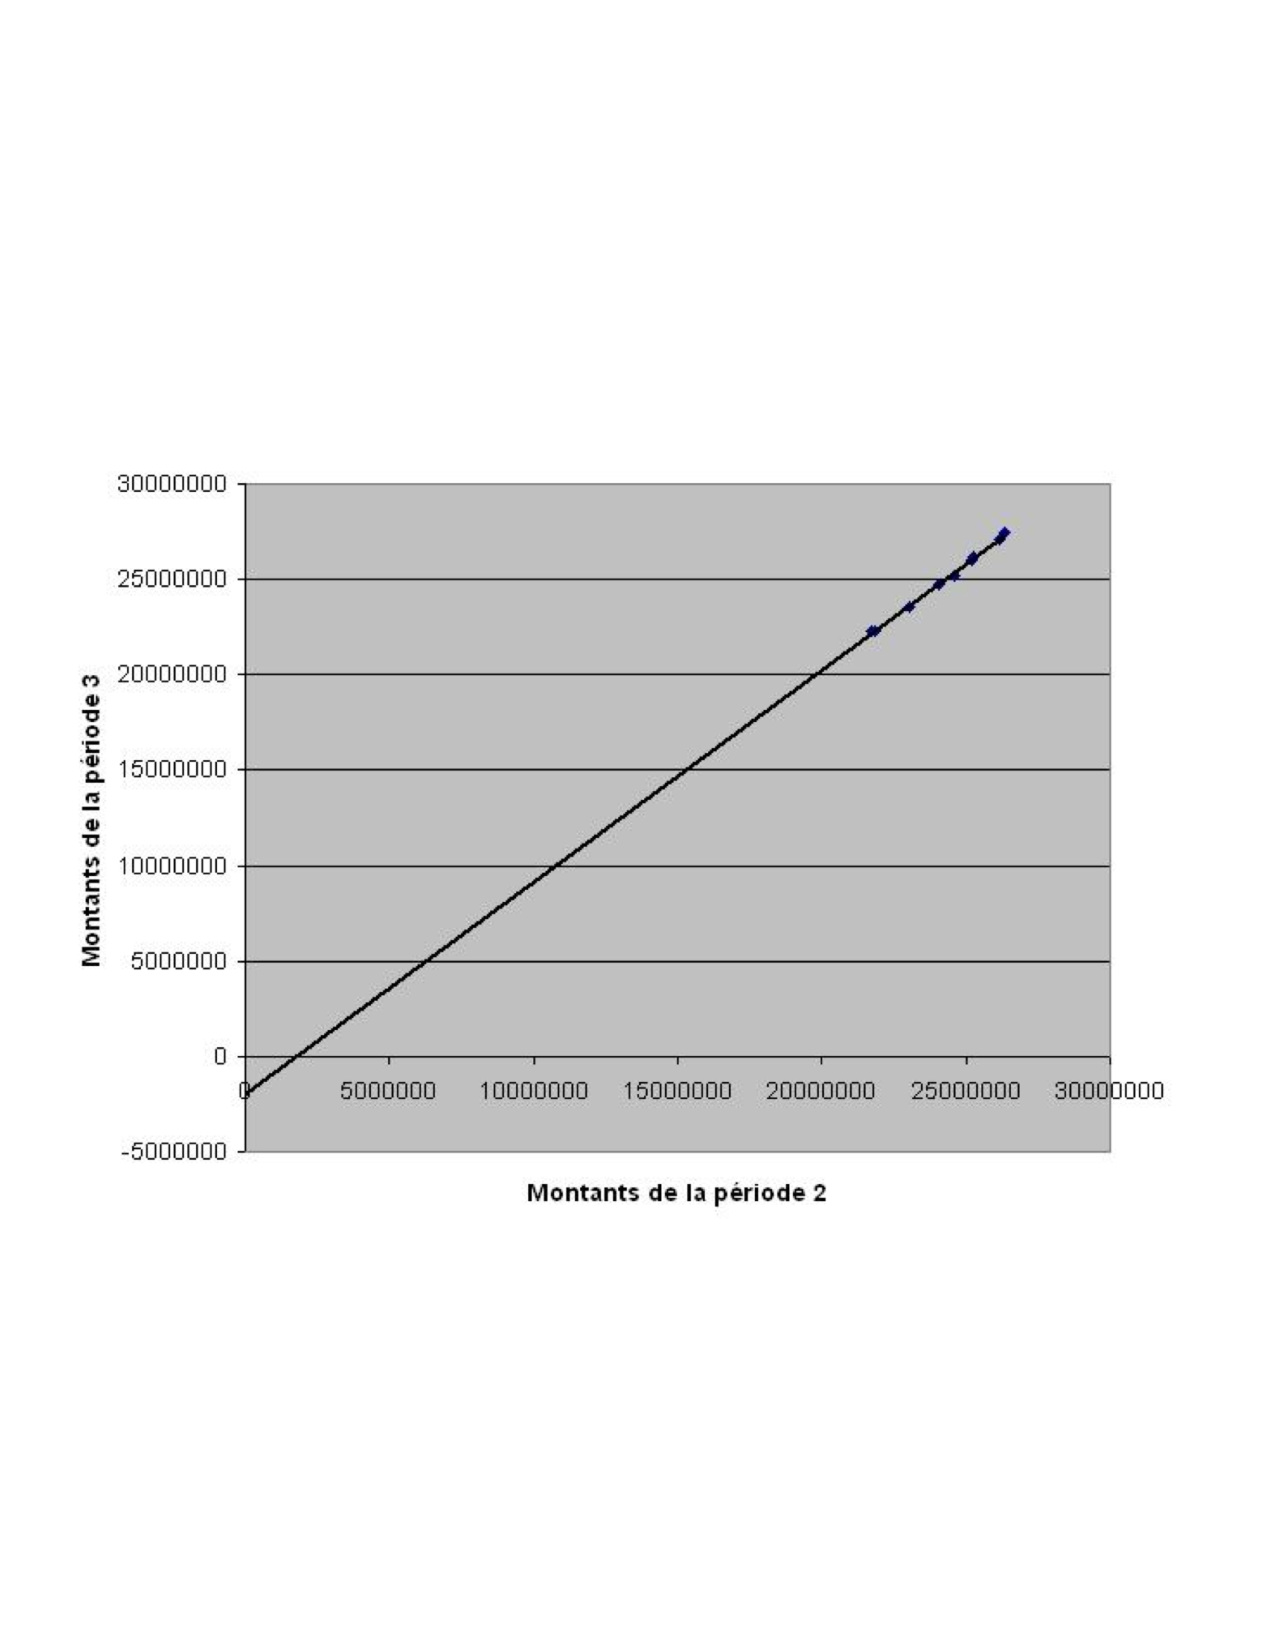
\includegraphics{images/H2}
  \caption{Droite des moindres carrés pour le nuage de points entre
    les périodes 2 et 3}
  \label{fig:deterministe:H2}
\end{figure}

Pour déterminer les paramètres de la droite, on utilise les moindres
carrés. Ainsi, on veut trouver les paramètres $\hat{\lambda}_j$ et
$\hat{\alpha}_j$ qui minimisent:
\begin{equation*}
  Q = \sum_{i=1}^{n-k} (C_{i,k+1} - \alpha_k - \lambda_k C_{i,k} )^2.
\end{equation*}
On a alors
\begin{align*}
  \frac{\delta Q}{\delta \alpha_k} &= \sum_{i=1}^{n-k} (C_{i,k+1} - \alpha_k - \lambda_k C_{i,k} ) = 0 \\
  \frac{\delta Q}{\delta \lambda_k} &= \sum_{i=1}^{n-k} C_{i,k} (C_{i,k+1} - \alpha_k - \lambda_k C_{i,k} ) = 0.
\end{align*}

\begin{align}
  \sum_{i=1}^{n-k} C_{i,k+1} - (n-k) \alpha_k - \lambda_k
  \sum_{i=1}^{n-k}  C_{i,k}
  &= 0 \label{eq:deterministe:eq1res} \\
  \sum_{i=1}^{n-k} C_{i,k} C_{i,k+1} -  \alpha_k \sum_{i=1}^{n-k}
  C_{i,k} - \lambda_k \sum_{i=1}^{n-k}  C_{i,k}^2
  &= 0. \label{eq:deterministe:eq2res}
\end{align}
En effectuant \eqref{eq:deterministe:eq2res} -
$\frac{\sum_{i=1}^{n-k} C_{i,k}}{n-k} \times$
\eqref{eq:deterministe:eq1res}, on obtient
\begin{align*}
  \frac{1}{n-k} \sum_{i=1}^{n-k} C_{i,k} C_{i,k+1} - \overline{C}_{k+1}^{(k)} \overline{C}_{k}^{(k)}
  &= \lambda_k \left(\frac{1}{n-k} \sum_{i=1}^{n-k}  C_{i,k}^2 - \overline{C}_{k}^{(k)} \overline{C}_{k}^{(k)} \right)
\end{align*}
\begin{align*}
  \hat{\lambda}_k &= \frac{\frac{1}{n-k} \sum_{i=1}^{n-k} C_{i,k} C_{i,k+1} - \overline{C}_{k+1}^{(k)} \overline{C}_{k}^{(k)} }
                    {\frac{1}{n-k} \sum_{i=1}^{n-k}  C_{i,k}^2 - \overline{C}_{k}^{(k)2} }
\end{align*}
avec
\begin{align*}
  \overline{C}_{k}^{(k)} &= \frac{1}{n-k}  \sum_{i=1}^{n-k} C_{i,k} \\
  \overline{C}_{k+1}^{(k)} &= \frac{1}{n-k} \sum_{i=1}^{n-k} C_{i,k+1}
\end{align*}
alors que
\begin{equation*}
  \hat{\alpha}_k = \overline{C}_{k+1}^{(k)} - \hat{\lambda}_k \overline{C}_{k}^{(k)}.
\end{equation*}

On note que $\alpha_{n}$ ne peut être calculé car on cherche à la fois
une tendance multiplicative et additive alors qu'il n'y a qu'un seul
couple d'observations. La convention veut que l'on ne considère que
l'effet multiplicatif pour cette dernière période de développement. Il
est généralement préférable d'utiliser la méthode London Chain
seulement s'il y a de bonnes raisons de croire qu'il y a un facteur
additif en plus d'un facteur multiplicatif dans le modèle.

\begin{exemple}
  Estimer les provisions avec la méthode London Chain
  \begin{center}
    \begin{tabular}{|l|l l l l l|}\hline
      Année & $1$ & $2$ & $3$ & $4$ & $5$  \\ \hline
      1997 &$\nombre{26312}$&	$\nombre{57779}$&	$\nombre{82451}$&	$\nombre{95506}$&	$\nombre{101604}$\\
      1998 &$\nombre{30470}$&	$\nombre{65482}$&	$\nombre{90973}$&	$\nombre{103562}$&	\\
      1999 &$\nombre{49756}$&	$\nombre{101587}$&	$\nombre{136854}$&	&	\\
      2000 &$\nombre{50420}$&	$\nombre{102735}$&	& &	\\
      2001 &$\nombre{56762}$&	&&&\\ \hline
    \end{tabular}
  \end{center}

  Évidemment, l'évaluation s'effectue beaucoup plus rapidement par
  ordinateur\dots\ On calcule $\alpha_1$ et $\lambda_1$ pour
  l'exemple:
  \begin{align*}
    \overline{C}_{1}^{(1)}
    &= \frac{1}{5-1}  \sum_{i=1}^{5-1} C_{i,1} \\
    &= \frac{\nombre{26312} +\nombre{30470}
      +\nombre{49756}+\nombre{50420}}{4} = \nombre{39239,5} \\
    \overline{C}_{1+1}^{(1)}
    &= \frac{1}{5-1} \sum_{i=1}^{5-1} C_{i,1+1} \\
    &= \frac{\nombre{57779}+\nombre{65482}+\nombre{101587}+\nombre{102735}}{4} = \nombre{81895,75}.
  \end{align*}
  \begin{align*}
    \hat{\lambda}_1
    &= \frac{\frac{1}{5-1} \sum_{i=1}^{5-1} C_{i,1} C_{i,1+1} - \overline{C}_{1+1}^{(1)} \overline{C}_{1}^{(1)} }
      {\frac{1}{5-1} \sum_{i=1}^{5-1}  C_{i,1}^2 - \overline{C}_{1}^{(1)2} }   \\
    &=   \frac{\frac{1}{4}(\nombre{26312}*\nombre{57779} + \nombre{30470}*\nombre{65482} + \nombre{49756}*\nombre{101587} + \nombre{50420}*\nombre{102735})  - \nombre{39239,5}*\nombre{81895,75} }
                      {\frac{1}{4} (\nombre{26312}^2+ \nombre{30470}^2 + \nombre{49756}^2 + \nombre{50420}^2) - \nombre{39239,5}^2}\\
    &= 1,86768.
  \end{align*}
  \begin{align*}
    \hat{\alpha}_1
    &= \overline{C}_{1+1}^{(1)} - \hat{\lambda}_1 \overline{C}_{1}^{(1)} \\
    &= \nombre{81895,75} - 1,86768 * \nombre{39239,5} \\
    &= \nombre{8608,88}.
  \end{align*}
  Au final, on obtient les résultats suivants:
  \begin{center}
    \begin{tabular}{|l|l l l l|}\hline
      k & $1 \rightarrow 2$ & $2 \rightarrow 3$ & $3 \rightarrow 4$ & $4 \rightarrow 5$   \\ \hline
      $\lambda_k$ & $1,86768$  & $1,3533$ & $1,1469$ & $1,0638$\\
      $\alpha_k$  & $\nombre{8608,92}$ & $\nombre{1495,52}$ & $42,21$ &\\ \hline
    \end{tabular}
  \end{center}
  Donc, si on complète le triangle, la dernière ligne est
  \begin{align*}
    \widehat{C}_{5,2}
    &= \nombre{8608,92} + 1,86768*\nombre{53762} = \nombre{109019} \\
    \widehat{C}_{5,3}
    &= \nombre{1495,52} + 1,3533*\nombre{109019} = \nombre{149031}\\
    & \dots
  \end{align*}
  \qed
\end{exemple}


\section{Méthode des provisions constituées}
\label{sec:deterministe:provisions-constituees}

Pour cette méthode, deux facteurs de projection sont utilisés: un pour
les paiements et un pour les provisions. La méthode Chain-Ladder
classique sur l'encouru total (qui correspond aux provisions
individuelles et aux paiements) suppose que les paiements et les
provisions se développent de manière identique. La méthode des
provisions constituées utilise davantage d'informations que le modèle
Chain-Ladder classique et est utile pour les branches à développement
très lentes, ou lorsque très peu de sinistres sont réglés la première
année.

\begin{description}
\item[Modèle pour les provisions] On note
  \begin{itemize}
  \item $Q_{i,j}$ est la provision pour les sinistres survenus au
    cours de l'année $i$, inscrite au passif du bilan en fin d'année
    $i+j-1$.
  \end{itemize}
  Le modèle est
  \begin{equation*}
    Q_{i, j+1} = k_{j+1} Q_{ij} - Y_{i, j+1},
  \end{equation*}
  où $k_{j+1}$ mesure la variation entre les années $j$ et $j+1$ de la
  prévision faite sur le coût total de sinistres survenus à l'année
  $i$.

  On estime $k_{j+1}$ :
  \begin{equation*}
    \hat{k}_{j+1} = \frac{\sum_{i=1}^{n-j} \left( Y_{i j+1} + Q_{i j+1} \right)}{\sum_{i=1}^{n-j} Q_{i j}}.
  \end{equation*}
  %
\item[Modèle pour les paiements] Le montant $Y_{i, j+1}$ payé au cours
  de l'année de développement $j+1$ est une fraction de $ Q_{ij}$:
  \begin{equation*}
    Y_{i, j+1} = h_{j+1}  Q_{ij}.
  \end{equation*}
  On estime $h_{j+1}$
  \begin{equation*}
    \hat{h}_{j+1} = \frac{\sum_{i=1}^{n-j} Y_{i j+1}}{\sum_{i=1}^{n-j} Q_{i j}}
  \end{equation*}
  %
\item[Extrapolation des triangles] Le triangle des paiements et des
  provisions sont complétés simultanément, diagonale par diagonale, en
  utilisant le formules précédentes l'une après l'autre.
  \begin{enumerate}
  \item On commence par la première diagonale inconnue des paiements:
    \begin{equation*}
      \hat{Y}_{i, n-i+2} = \hat{h}_{n-i+2}  Q_{i n-i+1} \text{ pour } i=2,\ldots,n.
    \end{equation*}
  \item On complète la première diagonale inconnue des provisions:
    \begin{equation*}
      \hat{Q}_{i, n-i+2} = k_{n-i+2} Q_{i n-i+1} - \hat{Y}_{i, n-i+2}
      \text{ pour } i=2, \ldots, n
    \end{equation*}
  \item On commence par l'autre diagonale inconnue des paiements.
  \item $\ldots$
  \end{enumerate}
\end{description}

On peut combiner ce modèle avec le modèle classique Chain-Ladder. En
combinant les équations des provisions et des paiements, on obtient
\begin{align*}
  Q_{i, j+1}
  &= k_{j+1} Q_{ij} - Y_{i, j+1}\\
  &= k_{j+1} Q_{ij} - h_{j+1}  Q_{ij} \\
  &= (k_{j+1} - h_{j+1}) Q_{ij} \\
  &= \left(\frac{\sum_{i=1}^{n-j} \left( Y_{i j+1} + Q_{i j+1} \right)}{\sum_{i=1}^{n-j} Q_{i j}}
    - \frac{\sum_{i=1}^{n-j} Y_{i j+1}}{\sum_{i=1}^{n-j} Q_{i j}} \right)  Q_{ij} \\
  &= \frac{\sum_{i=1}^{n-j} Q_{i j+1} }{\sum_{i=1}^{n-j} Q_{i j}}  Q_{ij},
\end{align*}
ce qui revient à la méthode Chain-Ladder. Cette méthode utilise plus
d'informations que la méthode Chain-Ladder, on peut donc choisir des
facteurs de développements différents pour les paiements et les
provisions (qui, elles, sont plus subjectives que les paiements - raison
fiscales, politiques, etc.).

\begin{exemple}
  Compléter les triangles de paiements et de provisions suivants:
  \begin{center}
    \begin{tabular}{|l|l l l l l|}\hline
      Année & $1$ & $2$ & $3$ & $4$ & $5$  \\ \hline
      1997 &$15,40$& $4,90$& $7,77$& $7,19$& $4,3$\\
      1998 &$16,61$& $2,60$& $11,03$& $9,12$& \\
      1999 &$21,35$& $7,29$& $5,59$& &\\
      2000 &$24,52$& $8,49$& & &\\
      2001 &$30,47$& & & &\\ \hline
    \end{tabular}
  \end{center}

  \begin{center}
    \begin{tabular}{|l|l l l l l|}\hline
      Année & $1$ & $2$ & $3$ & $4$ & $5$  \\ \hline
      1997 &$20,0$& $17,39$& $11,06$& $4,50$& $0,60$ \\
      1998 &$22,0$& $22,40$& $13,13$& $5,20$& \\
      1999 &$22,5$& $18,66$& $15,22$& & \\
      2000 &$25,0$& $20,32$& & &\\
      2001 &$25,0$&      & & & \\ \hline
    \end{tabular}
  \end{center}

  On a
  \begin{align*}
    \hat{k}_{1+1}
    &= \frac{\sum_{i=1}^{5-1} \left( Y_{i 1+1} + Q_{i 1+1} \right)}{\sum_{i=1}^{5-1} Q_{i 1}} \\
    &= \frac{17,39+4,90+22,4+2,6+18,66+7,29+20,32+8,49}{20,0+22,0+22,5+25,0} \\
    &= 1,1402\\
    \hat{k}_{3} &= 1,0915\\
    \hat{k}_{4} &= 1,0752\\
    \hat{k}_{5} &= 1,0889
  \end{align*}
  et
  \begin{align*}
    \hat{h}_{1+1}
    &= \frac{\sum_{i=1}^{5-1} Y_{i 1+1}}{\sum_{i=1}^{5-1} Q_{i 1}} \\
    &= \frac{4,90+2,6+7,29+8,49}{20,0+22,0+22,5+25,0} \\
    &= 0,2601 \\
    \hat{h}_{3} &= 0,4173\\
    \hat{h}_{4} &= 0,6742\\
    \hat{h}_{5} &= 0,9556.
  \end{align*}
  Et donc:
  \begin{center}
    \begin{tabular}{|l|l l l l l|}\hline
      Année & $1$ & $2$ & $3$ & $4$ & $5$  \\ \hline
      1997 &$15,40$& $4,90$& $7,77$& $7,19$& $4,3$\\
      1998 &$16,61$& $2,60$& $11,03$& $9,12$& $4,97$\\
      1999 &$21,35$& $7,29$& $5,59$& $10,26$& $5,83$\\
      2000 &$24,52$& $8,49$& $8,48$& $9,24$ &$5,25$\\
      2001 &$30,47$& $6,50$& $9,18$& $10,00$&$5,68$\\ \hline
    \end{tabular}
  \end{center}

  \begin{center}
    \begin{tabular}{|l|l l l l l|}\hline
      Année & $1$ & $2$ & $3$ & $4$ & $5$  \\ \hline
      1997 &$20,0$& $17,39$& $11,06$& $4,50$& $0,60$ \\
      1998 &$22,0$& $22,40$& $13,13$& $5,20$& $0,69$\\
      1999 &$22,5$& $18,66$& $15,22$& $6,10$& $0,81$\\
      2000 &$25,0$& $20,32$& $13,70$& $5,49$& $0,73$\\
      2001 &$25,0$& $22,0$ & $14,84$& $5,95$& $0,79$\\ \hline
    \end{tabular}
  \end{center}
  En sommant les provisions et les paiements, on obtient les encourus
  totaux. %
  \qed
\end{exemple}


\section{Méthode des moindres carrés de DeVylder}
\label{sec:deterministe:devylder}

Cette méthode est basée sur les incréments et non plus les montants
cumulatifs. Elle repose sur l'équation:
\begin{equation*}
  Y_{i,j} = r_j p_i,
\end{equation*}
où
\begin{itemize}
\item $p_i$ est la charge ultime des sinistres survenus l'années $i$;
  et
\item $r_j$ est la proportion du montant $p_i$ payé dans l'année de
  déroulement $j$.
\end{itemize}
Le triangle peut s'exprimer comme:

\begin{center}
  \begin{tabular}{|l l l l l|}\hline
    $r_1 p_1$ & $r_2 p_1$ & $\ldots$ & $r_{n-1} p_1$ & $r_n p_1$ \\
    $r_1 p_2$ & $r_2 p_2$ & $\ldots$ & $r_{n-1} p_2$ & \\
    $\ldots$ & $\ldots$ & $\ldots$ &  & \\
    $r_1 p_{n-1}$ & $r_2 p_{n-1}$ & &  & \\
    $r_1 p_n$ & & &  & \\ \hline
  \end{tabular}
\end{center}

Afin d'obtenir des estimateurs pour les paramètres inconnus, on
minimise la somme des carrés des écarts entre les valeurs observées
$Y_{ij}$ et leur forme théorique $r_j p_i$:
\begin{equation*}
  \sum_{i+j \le n } (Y_{i,j} - r_j p_i)^2
\end{equation*}
avec contrainte $r_1 + r_2 + \ldots + r_n = 1$. On obtient
\begin{align*}
  \hat{p}_{i} &= \frac{\sum_{j} \hat{r}_{j} Y_{i j}}{\sum_{j} \hat{r}_{j}^2 }\\
  \hat{r}_{j} &= \frac{\sum_{i} \hat{p}_{i} Y_{i j}}{\sum_{i} \hat{p}_{i}^2 }
\end{align*}
qu'il faut résoudre numériquement de manière récursive. Afin de
s'assurer que $r_1 + r_2 + \ldots + r_n = 1$, après chaque itération,
on peut diviser chaque nouveau $\hat{r}_{j}$ par la somme des nouveaux
$\hat{r}_{j}$.

\begin{exemple}
  On considère le triangle de paiement suivant:
  \begin{center}
    \begin{tabular}{|l|l l l l l|}\hline
      Année & $1$ & $2$ & $3$ & $4$ & $5$  \\ \hline
      1 (1997)& $\nombre{26312}$ & $\nombre{31467}$ & $\nombre{24672}$ & $\nombre{13055}$ & $\nombre{6158}$ \\
      2 (1998)& $\nombre{30470}$ & $\nombre{35012}$ & $\nombre{25491}$ & $\nombre{12589}$ &  \\
      3 (1999)& $\nombre{49756}$ & $\nombre{51831}$ & $\nombre{35267}$ &&\\
      4 (2000)& $\nombre{50420}$ & $\nombre{52315}$ & &&\\
      5 (2001)& $\nombre{56762}$ &  &&&\\ \hline
    \end{tabular}
  \end{center}
  Trouver la provision totale, si on a estimé que les $\hat{r}_{j}$
  (après convergence de l'algorithme) sont égaux à:
  \begin{center}
    \begin{tabular}{|l l l l l|}\hline
      $\hat{r}_1$ & $\hat{r}_2$ & $\hat{r}_3$ & $\hat{r}_4$ & $\hat{r}_5$ \\ \hline
      $0,2875$ &$0,3086$ &$0,2221$ &$0,1210$ &$0,0606$ \\ \hline
    \end{tabular}
  \end{center}
  Les $\hat{r}_{j}$ correspondent aux proportions annuelles payées de
  l'encouru total.

  \begin{align*}
    \hat{p}_{1} &= \frac{\sum_{j} \hat{r}_{j} Y_{1 j}}{\sum_{j} \hat{r}_{j}^2 }\\
                &= \frac{\nombre{26312}*0,2875 +\nombre{31467}*0,3086 + \nombre{24672}*0,2221 + \nombre{13055}*0,1210 + \nombre{6158}*0,0606}
                  {0,2875^2 + 0,3086^2 + 0,2221^2 + 0,1210^2 + 0,0606^2} \\
                &= \nombre{100603,22} \\
    \hat{p}_{2} &= \nombre{110585,90} \\
    \hat{p}_{3} &= \nombre{167806,52} \\
    \hat{p}_{4} &= \nombre{172235,48} \\
    \hat{p}_{5} &= \nombre{197480,59}.
  \end{align*}
  Donc, la provision revient à être $\hat{p}_j - C_{5-j+1,j}$!
  \begin{align*}
    \hat{p}_1 - C_{5,j} &= \nombre{101603,22} - \nombre{101604} \\
    \hat{p}_2 - C_{4,j} &= \nombre{110585,90} - \nombre{103562} \\
    \hat{p}_3 - C_{3,j} &= \nombre{167806,52} - \nombre{136854} \\
    \hat{p}_4 - C_{2,j} &= \nombre{172235,48} - \nombre{102735} \\
    \hat{p}_5 - C_{1,j} &= \nombre{197480,59} - \nombre{56762}.
  \end{align*}
  \qed
\end{exemple}


\section{Exercices}
\label{sec:prov:exercices}

\Opensolutionfile{reponses}[reponses-deterministe]
\Opensolutionfile{solutions}[solutions-deterministe]

\begin{Filesave}{reponses}
\bigskip
\section*{Réponses}

\end{Filesave}

\begin{Filesave}{solutions}
\section*{Chapitre \ref*{chap:deterministe}}
\addcontentsline{toc}{section}{Chapitre \protect\ref*{chap:deterministe}}

\end{Filesave}

\begin{exercice}
  Le \autoref{tab:deterministe:loss1} présente les différents
  paiements réalisés par l'assureur YTR.
  \begin{table}[!h]
    \centering
    \caption{Paiements réalisés par l'assureur YTR}
    \label{tab:deterministe:loss1}
    \begin{tabular}{cccc}
      \toprule
      Date paiement & Numéro assuré & Date survenance & Montant\\
      \midrule
      04/2000 & 456 & 03/2000 & $200$\\
      09/2000 & 476 & 08/2000 & $225$\\
      02/2001 & 456 & 03/2000 & $40$\\
      10/2001 & 476 & 08/2000 & $57$\\
      01/2002 & 456 & 03/2000 & $90$\\
      04/2003 & 476 & 08/2000 & $102$\\
      02/2004 & 476 & 08/2000 & $16$\\
      10/2001 & 287 & 10/2001 & $532$\\
      12/2002 & 287 & 10/2001 & $125$\\
      02/2003 & 937 & 03/2001 & $57$\\
      01/2004 & 287 & 10/2001 & $18$\\
      05/2002 & 456 & 03/2002 & $717$\\
      08/2003 & 456 & 03/2002 & $13$\\
      04/2004 & 456 & 03/2002 & $72$\\
      07/2003 & 101 & 07/2003 & $440$\\
      01/2004 & 867 & 03/2003 & $120$\\
      04/2004 & 200 & 02/2004 & $400$\\
      10/2004 & 956 & 08/2004 & $220$\\
      \bottomrule
    \end{tabular}
  \end{table}
  \begin{enumerate}
  \item Construire les triangles des paiements cumulés.
  \item Calculer les différents facteurs de développement. Discuter.
  \item Quel est le nombre de périodes nécessaires pour observer le
    développement complet des paiements?
  \item Déterminer le montant de provision nécessaire en utilisant la
    méthode Chain-Ladder.
  \item Un facteur de développement peut-il être inférieur à $1$?
  \end{enumerate}
  \begin{rep}
    \begin{enumerate}
      \stepcounter{enumi}
    \item $\lambda_1 = 1,167928$, $\lambda_2 = 1,114720$,
      $\lambda_3 = 1,090498$, $\lambda_4 = 1,022409$
    \item $5$
    \item $524$
    \item Oui
    \end{enumerate}
  \end{rep}
  \begin{sol}
    \begin{enumerate}
    \item Le triangle des paiements cumulés est présenté dans le
      tableau~\ref{tab:tri1}. Pour la case $(i, j)$, il suffit de
      sommer les montants des paiements pour les sinistres survenus
      pendant l'année~$i$ et payés pendant la $j\ieme$~période après
      la survenance.
      \begin{table}[!h]
        \centering
        \begin{tabular}{cccccc}
          \toprule
          & $1$ & $2$ & $3$ & $4$ & $5$\\
          \midrule
          2000 & $425$ & $522$ & $612$ & $714$ & $730$\\
          2001 & $532$ & $657$ & $714$ & $732$ & -\\
          2002 & $717$ & $730$ & $802$ & - & -\\
          2003 & $440$ & $560$ & - & - & -\\
          2004 & $620$ & - & - & - & -\\
          \bottomrule
        \end{tabular}
        \caption{Paiements réalisés par l'assureur YTR}
        \label{tab:tri1}
      \end{table}
    \item On a
      \begin{align*}
        \lambda_1 &= \frac{522 + 657 + 730 + 560}{425 + 532 + 717 + 440}\\
                  &=  \frac{\nombre{2469}}{\nombre{2114}}\\
                  &= 1,167928\\
        \lambda_2 &= \frac{\nombre{2128}}{\nombre{1909}}\\
                  &= 1,114720\\
        \lambda_3 &= \frac{\nombre{1446}}{\nombre{1326}}\\
                  &= 1,090498\\
        \lambda_4 &= \frac{\nombre{730}}{\nombre{714}}\\
                  &= 1,022409.
      \end{align*}
      Avant d'accepter aveuglément ces facteurs de développement, on
      peut analyser les facteurs de développement individuels (case
      par case) tels que présentés dans le tableau~\ref{tab:tri2}.
      Normalement, on devrait observer une certaine stabilité pour une
      même période de développement ($j$) entre les différentes années
      de survenance ($i$), ce qui n'est pas toujours le cas ici. Par
      exemple, on remarque que le passage de la période $1$ à la
      période $2$ est relativement stable pour les années 2000, 2001
      et 2003 (respectivement $1,23$, $1,23$ et $1,27$), un certain
      ralentissement dans la cadence des paiements est observé pour
      l'année 2002 ($1,02$). Après analyse, l'actuaire devra
      déterminer si ce ralentissement peut s'expliquer par un
      changement dans la politique de la compagnie pour cette année de
      survenance (et alors peut-être retirer les données de 2002 pour
      le calcul des facteurs de développement).
      \begin{table}[!h]
        \centering
        \begin{tabular}{ccccc}
          \toprule
          & $1-2$ & $2-3$ & $3-4$ & $4-5$\\
          \midrule
          2000 & $1,23$ & $1,17$ & $1,17$ & $1,02$\\
          2001 & $1,23$ & $1,09$ & $1,03$ & -\\
          2002 & $1,02$ & $1,10$ & - & -\\
          2003 & $1,27$ & - & - & -\\
          2004 & - & - & - & -\\
          \bottomrule
        \end{tabular}
        \caption{Facteurs de développement individuels}
        \label{tab:tri2}
      \end{table}
    \item Selon les données enregistrées par la compagnie, on observe
      un facteur de $1,02$ entre la $4\ieme$~période et la
      $5\ieme$~période de développement. Cette valeur étant très près
      de $1,00$, il est raisonnable de supposer que les paiements sont
      pratiquement complets après $5$~périodes de développement.
      Idéalement, le fait de pouvoir consulter une base de données
      semblables plus mature permettrait de confirmer ou d'infirmer
      cette hypothèse. Enfin, connaître le type de portefeuille
      (assurance automobile - dommage matériel, assurance automobile -
      dommage corporel, assurance responsabilité professionnelle,
      etc.) permettrait également d'avoir une idée du nombre de
      périodes de développement nécessaires.
    \item Le triangle complété des paiements cumulés est présenté dans
      le tableau~\ref{tab:tri3}. Par exemple,
      \begin{align*}
        (732)(1,022409) &= 748\\
        (802)(1,090498) &= 875\\
        (802)(1,090498)(1,022409) &= 894.
      \end{align*}
      \begin{table}[!h]
        \centering
        \begin{tabular}{cccccc}
          \toprule
          & $1$ & $2$ & $3$ & $4$ & $5$\\
          \midrule
          2000 & $425$ & $522$ & $612$ & $714$ & $730$\\
          2001 & $532$ & $657$ & $714$ & $732$ & $\textcolor{red}{748}$\\
          2002 & $717$ & $730$ & $802$ & $\textcolor{red}{875}$ & $\textcolor{red}{894}$\\
          2003 & $440$ & $560$ & $\textcolor{red}{624}$ & $\textcolor{red}{681}$ & $\textcolor{red}{696}$\\
          2004 & $620$ & $\textcolor{red}{724}$ & $\textcolor{red}{807}$ & $\textcolor{red}{880}$ & $\textcolor{red}{900}$\\
          \bottomrule
        \end{tabular}
        \caption{Paiements réalisés et estimés par l'assureur YTR}
        \label{tab:tri3}
      \end{table}
      Le montant total de la provision est donné par la différence entre
      le montant total des paiements ultimes et le montant total des
      paiements déjà réalisés:
      \begin{align*}
        730 + 748 + 894 + 696 + 900 &= \nombre{3968}\\
        730 + 732 + 802 + 560 + 620 &= \nombre{3444}\\
        \nombre{3968} - \nombre{3444} &= 524.
      \end{align*}
    \item Oui, c'est possible. Cela indiquerait que l'assureur a reçu
      des remboursements (paiements en trop, recours judiciaires,
      etc.).
    \end{enumerate}
  \end{sol}
\end{exercice}

\begin{exercice}
  L'actuaire de la compagnie GFR possède les informations suivantes
  sur les montants payés cumulatifs, en fonction des années de
  développement et de l'année de survenance du sinistre:
  \begin{center}
    \begin{tabular}{|l|l l l l l l l|}\hline
      Année & $1$ & $2$ & $3$ & $4$ & $5$ & $6$ & $7$\\ \hline
      1993 & $\nombre{1780}$ & $\nombre{2673}$ & $\nombre{2874}$ & $\nombre{3094}$ & $\nombre{3157}$ & $\nombre{3166}$ & $\nombre{3166}$ \\
      1994 & $\nombre{3226}$ & $\nombre{4219}$ & $\nombre{4532}$ & $\nombre{4881}$ & $\nombre{5144}$ & $\nombre{5199}$ & \\
      1995 & $\nombre{3652}$ & $\nombre{4989}$ & $\nombre{5762}$ & $\nombre{6436}$ & $\nombre{6720}$ & & \\
      1996 & $\nombre{2723}$ & $\nombre{4301}$ & $\nombre{5526}$ & $\nombre{6231}$ & & & \\
      1997 & $\nombre{2923}$ & $\nombre{4666}$ & $\nombre{5349}$ & & & & \\
      1998 & $\nombre{2990}$ & $\nombre{5417}$ & & & & & \\
      1999 & $\nombre{3917}$ & & & & & &\\ \hline
    \end{tabular}
  \end{center}
  En utilisant diverses variantes de la méthode Chain-Ladder, estimer
  les provisions pour ces données,
  \begin{enumerate}
  \item si on estime les facteurs de déroulement par la méthode
    \emph{Chain Ladder} usuelle;
  \item si on estime les facteurs de déroulement ($\lambda_j$) par une
    moyenne arithmétique;
  \item si on estime les facteurs de déroulement ($\lambda_j$) par une
    moyenne géométrique.
  \end{enumerate}
  \begin{rep}
    \begin{enumerate}
    \item $\nombre{7089}$
    \item $\nombre{6854}$
    \item $\nombre{6767}$
    \end{enumerate}
  \end{rep}
  \begin{sol}
    \begin{enumerate}
    \item On a
      \begin{align*}
        \lambda_1 &= \frac{\nombre{2673} + \nombre{4219} + \nombre{4989}
                    +\nombre{4301} + \nombre{4666} + \nombre{5417}}{\nombre{1780} +
                    \nombre{3226} + \nombre{3652} + \nombre{2723} + \nombre{2923} + \nombre{2990}}\\
                  &=  \frac{\nombre{26265}}{\nombre{17294}}\\
                  &= 1,518735\\
        \lambda_2 &=  1,153252\\
        \lambda_3 &= 1,104205\\
        \lambda_4 &=  1,042329\\
        \lambda_5 &= 1,007710\\
        \lambda_6 &= 1,000000.
      \end{align*}
      Le triangle complété est
      \begin{center}
        \begin{tabular}{|l|l l l l l l l|}\hline
          Année & $1$ & $2$ & $3$ & $4$ & $5$ & $6$ & $7$\\ \hline
          1993& $\nombre{1780}$& $\nombre{2673}$& $\nombre{2874}$& $\nombre{3094}$& $\nombre{3157}$& $\nombre{3166}$& $\nombre{3166}$ \\
          1994& $\nombre{3226}$& $\nombre{4219}$& $\nombre{4532}$& $\nombre{4881}$& $\nombre{5144}$& $\nombre{5199}$& $\nombre{5199}$ \\
          1995& $\nombre{3652}$& $\nombre{4989}$& $\nombre{5762}$& $\nombre{6436}$& $\nombre{6720}$& $\nombre{6772}$& $\nombre{6772}$ \\
          1996& $\nombre{2723}$& $\nombre{4301}$& $\nombre{5526}$& $\nombre{6231}$& $\nombre{6495}$& $\nombre{6545}$& $\nombre{6545}$ \\
          1997& $\nombre{2923}$& $\nombre{4666}$& $\nombre{5349}$& $\nombre{5906}$& $\nombre{6156}$& $\nombre{6204}$& $\nombre{6204}$ \\
          1998& $\nombre{2990}$& $\nombre{5417}$& $\nombre{6247}$& $\nombre{6898}$& $\nombre{7190}$& $\nombre{7246}$& $\nombre{7246}$ \\
          1999& $\nombre{3917}$& $\nombre{5949}$& $\nombre{6861}$& $\nombre{7575}$& $\nombre{7896}$& $\nombre{7957}$& $\nombre{7957}$\\\hline
        \end{tabular}
      \end{center}
      Le montant ultime payé est la somme de la dernière colonne,
      $\nombre{43088}$, et le montant de la provision est la
      différence entre le montant ultime et le montant total payé
      (somme de la diagonale principale):
      $\nombre{43088} - \nombre{35999} = \nombre{7089}$.
    \item On calcule, pour chaque cellule, le facteur de développement
      \begin{center}
        \begin{tabular}{|l|l l l l l l|}\hline
          Année & 1$\rightarrow$ 2 &  2$\rightarrow$ 3 &  3$\rightarrow$ 4 &
                                                                             4$\rightarrow$ 5 & 5$\rightarrow$ 6 & 6$\rightarrow$ 7 \\ \hline
          1993 &$1,501685$&$1,075196$&$1,076548$&$1,020362$&$1,002851$ & $1$\\
          1994 &$1,307812$&$1,074188$&$1,077008$&$1,053882$&$1,010692$ & $$\\
          1995 &$1,366101$&$1,154941$&$1,116973$&$1,044127$&$$ & $$\\
          1996 &$1,579508$&$1,284817$&$1,127579$& & & \\
          1997 &$1,596305$&$1,146378$& & & & \\
          1998 &$1,811706$& &&& & \\\hline
          Moy. arith. &$1,527186$&$1,147104$&$1,099527$&$1,039457$ & $1,006771$ & $1$\\\hline
        \end{tabular}
      \end{center}
      Le triangle complété est
      \begin{center}
        \begin{tabular}{|l|l l l l l l l|}\hline
          Année & $1$ & $2$ & $3$ & $4$ & $5$ & $6$ & $7$\\ \hline
          1993& $\nombre{1780}$& $\nombre{2673}$& $\nombre{2874}$& $\nombre{3094}$& $\nombre{3157}$& $\nombre{3166}$& $\nombre{3166}$ \\
          1994& $\nombre{3226}$& $\nombre{4219}$& $\nombre{4532}$& $\nombre{4881}$& $\nombre{5144}$& $\nombre{5199}$& $\nombre{5199}$ \\
          1995& $\nombre{3652}$& $\nombre{4989}$& $\nombre{5762}$& $\nombre{6436}$& $\nombre{6720}$& $\nombre{6766}$& $\nombre{6766}$ \\
          1996& $\nombre{2723}$& $\nombre{4301}$& $\nombre{5526}$& $\nombre{6231}$& $\nombre{6477}$& $\nombre{6521}$& $\nombre{6521}$ \\
          1997& $\nombre{2923}$& $\nombre{4666}$& $\nombre{5349}$& $\nombre{5881}$& $\nombre{6113}$& $\nombre{6155}$& $\nombre{6155}$ \\
          1998& $\nombre{2990}$& $\nombre{5417}$& $\nombre{6214}$& $\nombre{6832}$& $\nombre{7102}$& $\nombre{7150}$& $\nombre{7150}$ \\
          1999& $\nombre{3917}$& $\nombre{5982}$& $\nombre{6862}$& $\nombre{7545}$& $\nombre{7843}$& $\nombre{7896}$& $\nombre{7896}$\\\hline
        \end{tabular}
      \end{center}
      Le montant ultime payé est la somme de la dernière colonne,
      $\nombre{42853}$, et le montant de la provision est la
      différence entre le montant ultime et le montant total payé
      (somme de la diagonale principale): $\nombre{42853} -
      \nombre{35999} = \nombre{6854}$.
    \item On calcule, pour chaque cellule, le facteur de développement
      \begin{center}
        \begin{tabular}{|l|l l l l l l|}\hline
          Année & 1$\rightarrow$ 2 &  2$\rightarrow$ 3 &  3$\rightarrow$ 4 &
                                                                             4$\rightarrow$ 5 & 5$\rightarrow$ 6 & 6$\rightarrow$ 7 \\ \hline
          1993 &$1,501685$&$1,075196$&$1,076548$&$1,020362$&$1,002851$ & $1$\\
          1994 &$1,307812$&$1,074188$&$1,077008$&$1,053882$&$1,010692$ & $$\\
          1995 &$1,366101$&$1,154941$&$1,116973$&$1,044127$&$$ & $$\\
          1996 &$1,579508$&$1,284817$&$1,127579$& & & \\
          1997 &$1,596305$&$1,146378$& & & & \\
          1998 &$1,811706$& &&& & \\\hline
          Moy. géo. &$1,518409$&$1,144615$&$1,099286$&$1,039361$ & $1,006764$ & $1$\\\hline
        \end{tabular}
      \end{center}
      Le triangle complété est
      \begin{center}
        \begin{tabular}{|l|l l l l l l l|}\hline
          Année & $1$ & $2$ & $3$ & $4$ & $5$ & $6$ & $7$\\ \hline
          1993& $\nombre{1780}$& $\nombre{2673}$& $\nombre{2874}$& $\nombre{3094}$& $\nombre{3157}$& $\nombre{3166}$& $\nombre{3166}$ \\
          1994& $\nombre{3226}$& $\nombre{4219}$& $\nombre{4532}$& $\nombre{4881}$& $\nombre{5144}$& $\nombre{5199}$& $\nombre{5199}$ \\
          1995& $\nombre{3652}$& $\nombre{4989}$& $\nombre{5762}$& $\nombre{6436}$& $\nombre{6720}$& $\nombre{6765}$& $\nombre{6765}$ \\
          1996& $\nombre{2723}$& $\nombre{4301}$& $\nombre{5526}$& $\nombre{6231}$& $\nombre{6476}$& $\nombre{6520}$& $\nombre{6520}$ \\
          1997& $\nombre{2923}$& $\nombre{4666}$& $\nombre{5349}$& $\nombre{5880}$& $\nombre{6112}$& $\nombre{6153}$& $\nombre{6153}$ \\
          1998& $\nombre{2990}$& $\nombre{5417}$& $\nombre{6200}$& $\nombre{6816}$& $\nombre{7084}$& $\nombre{7132}$& $\nombre{7132}$ \\
          1999& $\nombre{3917}$& $\nombre{5948}$& $\nombre{6808}$& $\nombre{7484}$& $\nombre{7778}$& $\nombre{7831}$& $\nombre{7831}$\\\hline
        \end{tabular}
      \end{center}
      Le montant ultime payé est la somme de la dernière colonne,
      $\nombre{42766}$, et le montant de la provision est la
      différence entre le montant ultime et le montant total payé
      (somme de la diagonale principale):
      $\nombre{42766} - \nombre{35999} = \nombre{6767}$.
    \end{enumerate}
  \end{sol}
\end{exercice}

\begin{exercice}
  L'actuaire de la compagnie \emph{Dujardin et cie} a collecté les
  informations suivantes sur les montants payés par année $Y_{i,j}$,
  en fonction des années de développement et de l'année de survenance
  du sinistre
  \begin{center}
    \begin{tabular}{|c|c c c c c c|}\hline
      Année & $1$ & $2$ & $3$ & $4$ & $5$ & $6$ \\ \hline
      1994 & $192$ & $251$ & $153$ & $145$ & $98$  & $0$ \\
      1995 & $205$ & $280$ & $195$ & $150$ & $102$ &   \\
      1996 & $230$ & $345$ & $230$ & $212$ &     &   \\
      1997 & $288$ & $410$ & $275$ &     &     &   \\
      1998 & $398$ & $563$ &     &     &     &   \\
      1999 & $530$ &     &     &     &     &   \\ \hline
    \end{tabular}
  \end{center}
  Estimer les provisions pour ces données si on estime les facteurs de
  déroulement par la méthode Chain-Ladder usuelle.
  \begin{rep}
    $\nombre{3382}$
  \end{rep}
  \begin{sol}
    On construit premièrement le triangle des valeurs cumulées
    \begin{center}
      \begin{tabular}{|c|c c c c c c|}\hline
        Année & $1$ & $2$ & $3$ & $4$ & $5$ & $6$ \\ \hline
        1994 & $192$ & $443$ & $596$ & $741$ & $839$  & $839$ \\
        1995 & $205$ & $485$ & $680$ & $830$ & $932$ &   \\
        1996 & $230$ & $575$ & $805$ & $\nombre{1017}$ &     &   \\
        1997 & $288$ & $698$ & $973$ &     &     &   \\
        1998 & $398$ & $961$ &     &     &     &   \\
        1999 & $530$ &     &     &     &     &   \\ \hline
      \end{tabular}
    \end{center}
    On a
    \begin{align*}
      \lambda_1 &= \frac{\nombre{443} + \nombre{485} + \nombre{575}
                  +\nombre{698} + \nombre{961}}{\nombre{192} +
                  \nombre{205} + \nombre{230} + \nombre{288} + \nombre{398}}\\
                &=  \frac{\nombre{3162}}{\nombre{1313}}\\
                &= 2,408225\\
      \lambda_2 &=  1,387551\\
      \lambda_3 &= 1,243633\\
      \lambda_4 &=  1,127307\\
      \lambda_5 &= 1,000000.
    \end{align*}
    Le triangle complété est
    \begin{center}
      \begin{tabular}{|c|c c c c c c|}\hline
        Année & $1$ & $2$ & $3$ & $4$ & $5$ & $6$ \\ \hline
        1994 & $192$ & $443$ & $596$ & $741$ & $839$  & $839$ \\
        1995 & $205$ & $485$ & $680$ & $830$ & $932$ & $932$  \\
        1996 & $230$ & $575$ & $805$ & $\nombre{1017}$ & $\nombre{1146}$    & $\nombre{1146}$  \\
        1997 & $288$ & $698$ & $973$ &  $\nombre{1210}$   &   $\nombre{1364}$  & $\nombre{1364}$  \\
        1998 & $398$ & $961$ &  $\nombre{1333}$   &  $\nombre{1658}$   & $\nombre{1869}$    & $\nombre{1869}$  \\
        1999 & $530$ &  $\nombre{1276}$   &  $\nombre{1771}$   &   $\nombre{2202}$  &  $\nombre{2483}$   &  $\nombre{2483}$ \\ \hline
      \end{tabular}
    \end{center}
    Le montant ultime payé est la somme de la dernière colonne,
    $\nombre{8634}$, et le montant de la provision est la différence
    entre le montant ultime et le montant total payé (somme de la
    diagonale principale):
    $\nombre{8634} - \nombre{5252} = \nombre{3382}$.
  \end{sol}
\end{exercice}

\begin{exercice}
  Pour une certaine années d'accident, on a les informations
  suivantes:
  \begin{itemize}
  \item primes acquises : $\nombre{1000}$~\$;
  \item rapport Sinistres/Primes espéré : $0,650$;
  \item $\prod_{k=2}^{ult} \lambda_k = 1,12$;
  \item sinistres encourus à ce jour: $600$~\$; et
  \item sinistres payés à ce jour: $500$~\$.
  \end{itemize}
  Calculer l'estimation des montants des provisions en utilisant la
  technique de Bornhuetter-Ferguson.
  \begin{rep}
    $69,64286$
  \end{rep}
  \begin{sol}
    \begin{align*}
      \hat{C}_{i}^{LR} &= \Esp{LR} \times \text{Primes acquises}_i\\
                       &= 0,650 * \nombre{1000} = \nombre{650} \\
      R_i^{BF} &= \hat{C}_{i}^{LR} \times ( 1 - \frac{1}{\prod_{k=2}^{\infty} \lambda_k}) \\
                       &= \nombre{650} (1-\frac{1}{1,12}) = \nombre{69,64286}.
    \end{align*}
  \end{sol}
\end{exercice}

\begin{exercice}
  On suppose qu'on a estimé les facteurs de développement par la
  méthode Chain-Ladder usuelle et qu'on a obtenu
  \begin{center}
    \begin{tabular}{|c c c c c|}\hline
      1$\rightarrow$ 2 &  2$\rightarrow$ 3 &  3$\rightarrow$ 4 &  4$\rightarrow$ 5  &5 $\rightarrow  \infty$  \\ \hline
      $1,75$ & $1,6$ & $1,4$ & $1,1$ & $1,05$ \\ \hline
    \end{tabular}
  \end{center}
  \begin{itemize}
  \item Pour l'année 1998, on estime le 31/12/1999 des paiements
    cumulatifs de $\nombre{320000}$~\$;
  \item les primes acquises de 1998 sont de $\nombre{1000000}$~\$; et
  \item le rapport sinistres/primes espéré de l'année 1998 est de
    $0,650$.
  \end{itemize}
  Estimer les provisions pour l'année d'accident 1998:
  \begin{enumerate}
  \item en utilisant la méthode du rapport sinistres/primes espéré;
  \item en utilisant la méthode Chain-Ladder; et
  \item en utilisant la méthode Bornhuetter-Ferguson.
  \end{enumerate}
  \begin{rep}
    \begin{enumerate}
    \item $\nombre{330000}$
    \item $\nombre{507904}$
    \item $\nombre{398763,1}$
    \end{enumerate}
  \end{rep}
  \begin{sol}
    La première évaluation des provisions de l'année d'accident 1998 est
    le 31 décembre 1998. Ainsi, le 31 décembre 1999, on est à la
    deuxième évaluation.
    \begin{enumerate}
    \item On a
      \begin{align*}
        \underbrace{\hat{C}_{i}^{LR}}_{\text{Pertes ultimes attendues selon LR}} &=
                                                                                   \underbrace{\Esp{LR}}_{\text{Rapport sinistres/primes espéré}} \times \text{Primes acquises}_i\\
                                                                                 &= 0,650 * \nombre{1000000} = \nombre{650000} \\
        \underbrace{R_i^{LR}}_{\text{Provisions selon la méthode du rapport sinistres/primes}}
                                                                                 &= \hat{C}_{i}^{LR} - \underbrace{C_{i, 2}}_{\text{Paiements cumulatifs à la deuxième évaluation}} \\
                                                                                 &= \nombre{650000} - \nombre{320000} = \nombre{330000}.
      \end{align*}

    \item On a
      \begin{align*}
        \underbrace{\hat{C}_{i}^{CL}}_{\text{Pertes ultimes attendues selon CL}} &=
                                                                                   C_{i, 2} \times (\prod_{k=2}^{\infty} \lambda_k)\\
                                                                                 &= \nombre{320000} \times  1,60 * 1,40 * 1,10 * 1,05 \\
                                                                                 &= \nombre{320000} * 2,5872 = \nombre{827904}\\
        \underbrace{R_i^{CL}}_{\text{Provisions selon la méthode CL}}
                                                                                 &= \hat{C}_{i}^{CL} - C_{i, 2} \\
                                                                                 &= \nombre{827904} - \nombre{320000} = \nombre{507904}.
      \end{align*}

    \item On a
      \begin{align*}
        R_i^{BF} &= \hat{C}_{i}^{LR} \times ( 1 - \frac{1}{\prod_{k=2}^{\infty} \lambda_k}) \\
                 &= \nombre{650000} (1-\frac{1}{2,5872}) = \nombre{398763,1}.
      \end{align*}
    \end{enumerate}
  \end{sol}
\end{exercice}

\begin{exercice}
  On suppose qu'on a estimé les facteurs de développement par la
  méthode Chain-Ladder
  \begin{center}
    \begin{tabular}{|c c c c c c|}\hline
      1$\rightarrow$ 2 &  2$\rightarrow$ 3 &  3$\rightarrow$ 4 &  4$\rightarrow$ 5  &5 $\rightarrow$ 6 &6 $\rightarrow  \infty$ \\ \hline
      $1,55$ & $1,5$ & $1,3$ & $1,25$ & $1,15$ & $1,05$ \\ \hline
    \end{tabular}
  \end{center}
  \begin{itemize}
  \item Pour l'année 1999, on estime le 31/12/1999 des paiements
    cumulatifs de $\nombre{120000}$~\$;
  \item les primes acquises de 1999 sont de $\nombre{1350000}$~\$; et
  \item le rapport sinistres/primes espéré de l'année 1999 est de
    $0,600$.
  \end{itemize}
  Estimer les provisions pour l'année d'accident 1999:
  \begin{enumerate}
  \item en utilisant la méthode du rapport sinistres/primes espéré;
  \item en utilisant la méthode Chain-Ladder; et
  \item en utilisant la méthode Bornhuetter Ferguson.
  \item Le 31/12/2002, les paiements cumulatifs sont maintenant de
    $\nombre{200000}$~\$. Pour les trois méthodes précédentes,
    calculer la différence entre la réalisation et la projection.
  \item Quel est l'avantage d'utiliser la méthode de
    Bornhuetter-Ferguson par rapport à celle de Chain-Ladder ?
  \end{enumerate}
  \begin{rep}
    \begin{enumerate}
    \item $\nombre{690000}$
    \item $\nombre{427450,3}$
    \item $\nombre{632449,6}$
    \item $\nombre{162700}$ et $\nombre{73354}$
    \end{enumerate}
  \end{rep}
  \begin{sol}
    \begin{enumerate}
    \item On a
      \begin{align*}
        \underbrace{\hat{C}_{i}^{LR}}_{\text{Pertes ultimes attendues selon LR}} &=
                                                                                   \underbrace{\Esp{LR}}_{\text{Rapport sinistres/primes espéré}} \times \text{Primes acquises}_i\\
                                                                                 &= 0,600 * \nombre{1350000} = \nombre{810000} \\
        \underbrace{R_i^{LR}}_{\text{Provisions selon la méthode du rapport sinistres/primes}}
                                                                                 &= \hat{C}_{i}^{LR} - \underbrace{C_{i, 1}}_{\text{Paiements cumulatifs à la première évaluation}} \\
                                                                                 &= \nombre{810000} - \nombre{120000} = \nombre{690000}.
      \end{align*}

    \item On a
      \begin{align*}
        \underbrace{\hat{C}_{i}^{CL}}_{\text{Pertes ultimes attendues selon CL}} &=
                                                                                   C_{i, 1} \times (\prod_{k=1}^{\infty} \lambda_k)\\
                                                                                 &= \nombre{120000} \times  1,55 * 1,50 * 1,30 * 1,25 * 1,05 \\
                                                                                 &=
                                                                                   \nombre{120000}
                                                                                   *
                                                                                   4,562086
                                                                                   =
                                                                                   \nombre{547450,3}
        \\
        \underbrace{R_i^{CL}}_{\text{Provisions selon la méthode CL}}
                                                                                 &= \hat{C}_{i}^{CL} - C_{i, 1} \\
                                                                                 &= \nombre{547450,3} - \nombre{120000} = \nombre{427450,3}.
      \end{align*}

    \item On a
      \begin{align*}
        R_i^{BF} &= \hat{C}_{i}^{LR} \times ( 1 - \frac{1}{\prod_{k=1}^{\infty} \lambda_k}) \\
                 &= \nombre{810000} (1-\frac{1}{4,562086}) = \nombre{632449,6}.
      \end{align*}
    \item Pour la première méthode, il n'est pas possible de ventiler
      les provisions. Pour la méthode Chain-Ladder, on a
      \begin{align*}
        \nombre{120000} \times 1,55 * 1,50 * 1,30 &= \nombre{362700}\\
        \Delta &= \nombre{362700} - \nombre{200000} = \nombre{162700}.
      \end{align*}
      Pour la méthode BF, on a
      \begin{itemize}
      \item du temps 1 au temps $\infty$, le facteur de développement
        est de $1,55 * 1,50 * 1,30 * 1,25 * 1,15 * 1,05 = 4,562086$;
      \item du temps 2 au temps $\infty$, le facteur de développement
        est de $1,50 * 1,30 * 1,25 * 1,15 * 1,05 = 2,943281$;
      \item du temps 3 au temps $\infty$, le facteur de développement
        est de $1,30 * 1,25 * 1,15 * 1,05 = 1,962187$;
      \item du temps 4 au temps $\infty$, le facteur de développement
        est de $1,25 * 1,15 * 1,05 = 1,509375$;
      \item du temps 5 au temps $\infty$, le facteur de développement
        est de $1,15 * 1,05 = 1,207500$; et
      \item du temps 6 au temps $\infty$, le facteur de développement
        est de $1,05$.
      \end{itemize}
      Ainsi:
      \begin{center}
        \begin{tabular}{|c|c|c|}\hline
          Date ($j$) & $\hat{C}_{i,j}^{BF}$ & $\hat{Y}_{i,j}^{BF}$  \\ \hline
          Décembre 2000 &  $\nombre{217652,72}$ & $\nombre{97652,72}$ \\ \hline
          Décembre 2001 &  $\nombre{355254,3}$ & $\nombre{137601,6}$\\ \hline
          Décembre 2002 &  $\nombre{479095,6}$ & $\nombre{123841,3}$\\ \hline
        \end{tabular}
      \end{center}
    \item La méthode BF permet de stabiliser la provision par rapport à
      la méthode Chain-Ladder, en particulier pour les périodes
      récentes.
    \end{enumerate}
  \end{sol}
\end{exercice}

\begin{exercice}
  En utilisant le triangle des paiements cumulatifs suivants
  \begin{center}
    \begin{tabular}{|c|c c c c c c c|}\hline
      Année & $1$ & $2$ & $3$ & $4$ & $5$ & $6$ & $7$\\ \hline
      1993 & $\nombre{1780}$ & $\nombre{2673}$ & $\nombre{2874}$ & $\nombre{3094}$ & $\nombre{3157}$ & $\nombre{3166}$ & $\nombre{3166}$ \\
      1994 & $\nombre{3226}$ & $\nombre{4219}$ & $\nombre{4532}$ & $\nombre{4881}$ & $\nombre{5144}$ & $\nombre{5199}$ & \\
      1995 & $\nombre{3652}$ & $\nombre{4989}$ & $\nombre{5762}$ & $\nombre{6436}$ & $\nombre{6720}$ & & \\
      1996 & $\nombre{2723}$ & $\nombre{4301}$ & $\nombre{5526}$ & $\nombre{6231}$ & & & \\
      1997 & $\nombre{2923}$ & $\nombre{4666}$ & $\nombre{5349}$ & & & & \\
      1998 & $\nombre{2990}$ & $\nombre{5417}$ & & & & & \\
      1999 & $\nombre{3917}$ & & & & & &\\ \hline
    \end{tabular}
  \end{center}
  répondre à la question suivante.
  \begin{enumerate}
  \item Déterminer la provision pour l'année d'accident 1998 par la
    méthode Chain-Ladder.
  \item Déterminer la provision pour les années d'accident 1998 par la
    méthode London Chain.
  \item Pourquoi peut-on dire que la méthode London Chain inclut la
    méthode Chain Ladder?
  \end{enumerate}
  \begin{rep}
    \begin{enumerate}
    \item $\nombre{1829}$
    \item $\nombre{1854,575}$
    \end{enumerate}
  \end{rep}
  \begin{sol}
    \begin{enumerate}
    \item On a
      \begin{align*}
        \lambda_1 &= \frac{\nombre{2673} + \nombre{4219} + \nombre{4989}
                    +\nombre{4301} + \nombre{4666} + \nombre{5417}}{\nombre{1780} +
                    \nombre{3226} + \nombre{3652} + \nombre{2723} + \nombre{2923} + \nombre{2990}}\\
                  &=  \frac{\nombre{26265}}{\nombre{17294}}\\
                  &= 1,518735\\
        \lambda_2 &=  1,153252\\
        \lambda_3 &= 1,104205\\
        \lambda_4 &=  1,042329\\
        \lambda_5 &= 1,007710\\
        \lambda_6 &= 1,000000.
      \end{align*}
      Le triangle complété est
      \begin{center}
        \begin{tabular}{|l|l l l l l l l|}\hline
          Année & $1$ & $2$ & $3$ & $4$ & $5$ & $6$ & $7$\\ \hline
          1993& $\nombre{1780}$& $\nombre{2673}$& $\nombre{2874}$& $\nombre{3094}$& $\nombre{3157}$& $\nombre{3166}$& $\nombre{3166}$ \\
          1994& $\nombre{3226}$& $\nombre{4219}$& $\nombre{4532}$& $\nombre{4881}$& $\nombre{5144}$& $\nombre{5199}$& $\nombre{5199}$ \\
          1995& $\nombre{3652}$& $\nombre{4989}$& $\nombre{5762}$& $\nombre{6436}$& $\nombre{6720}$& $\nombre{6772}$& $\nombre{6772}$ \\
          1996& $\nombre{2723}$& $\nombre{4301}$& $\nombre{5526}$& $\nombre{6231}$& $\nombre{6495}$& $\nombre{6545}$& $\nombre{6545}$ \\
          1997& $\nombre{2923}$& $\nombre{4666}$& $\nombre{5349}$& $\nombre{5906}$& $\nombre{6156}$& $\nombre{6204}$& $\nombre{6204}$ \\
          1998& $\nombre{2990}$& $\nombre{5417}$& $\nombre{6247}$& $\nombre{6898}$& $\nombre{7190}$& $\nombre{7246}$& $\nombre{7246}$ \\
          1999& $\nombre{3917}$& $\nombre{5949}$& $\nombre{6861}$& $\nombre{7575}$& $\nombre{7896}$& $\nombre{7957}$& $\nombre{7957}$\\\hline
        \end{tabular}
      \end{center}
      Pour 1998, le montant ultime payé est $\nombre{7246}$, et le
      montant de la provision est la différence entre le montant ultime
      et le montant total payé:
      $\nombre{7246} - \nombre{5417} = \nombre{1829}$.
    \item On a
      \begin{align*}
        \overline{C}_k^{(k)} &= \frac{1}{n - k}\sum_{i=1}^{n-k}C_{i,k}\\
        \overline{C}_1^{(1)} &=
                               \frac{(\nombre{1780}+\nombre{3226}+\nombre{3652}+\nombre{2723}+\nombre{2923}+\nombre{2990})}{7-1}\\
                             &= \nombre{2882,33} \\
        \overline{C}_2^{(2)} &= \nombre{4169,6} \\
        \overline{C}_3^{(3)} &= \nombre{4673,5} \\
        \overline{C}_4^{(4)} &= \nombre{4803,67} \\
        \overline{C}_5^{(5)} &= \nombre{4150,5} \\
        \overline{C}_6^{(6)} &= \nombre{3166}
      \end{align*}
      \begin{align*}
        \overline{C}_{k+1}^{(k)} &= \frac{1}{n-k} \sum_{i=1}^{n-k}
                                   C_{i,k+1}\\
        \overline{C}_2^{(1)} &=
                               \frac{(\nombre{2673}+\nombre{4219}+\nombre{4989}+\nombre{4301}+\nombre{4666}+\nombre{5417})}{7-1}\\
                                 &= \nombre{4377,5} \\
        \overline{C}_3^{(2)} &= \nombre{4808,6} \\
        \overline{C}_4^{(3)} &= \nombre{5160,5} \\
        \overline{C}_5^{(4)} &= \nombre{5007} \\
        \overline{C}_6^{(5)} &= \nombre{4182,5} \\
        \overline{C}_7^{(6)} &= \nombre{3166}
      \end{align*}
      \begin{align*}
        \hat{\lambda}_1 &= \frac{\frac{1}{7-1} \sum_{i=1}^{7-1} C_{i,1} C_{i,2} - \overline{C}_{2}^{(1)} \overline{C}_{1}^{(1)}}
                          {\frac{1}{7-1} \sum_{i=1}^{7-1}  C_{i,1}^2 - \overline{C}_{1}^{(1)2} }   \\
                        &=   \frac{\frac{1}{6}(\nombre{1780}*\nombre{2673} +
                          \nombre{3226}*\nombre{4219} + \ldots + \nombre{2990}*\nombre{5417})  - \nombre{2882,33}*\nombre{4377,5}}
                          {\frac{1}{6} (\nombre{1780}^2+ \nombre{3226}^2 + \nombre{3652}^2 + \nombre{2723}^2+ \nombre{2923}^2+ \nombre{2990}^2) - \nombre{2882,33}^2}\\
                        &= \frac{\nombre{13022572} -
                          \nombre{12617400}}{\nombre{8635223} - \nombre{7965547}}\\
                        &= 0,6050274\\
        \hat{\lambda}_2 &= 1,266904\\
        \hat{\lambda}_3 &= 1,172035\\
                        &\ldots
      \end{align*}
      \begin{align*}
        \hat{\alpha}_1 &= \overline{C}_{2}^{(1)} -
                         \hat{\lambda}_1\overline{C}_1^{(1)}\\
                       &= \nombre{4377,5} - (0,6050274)(\nombre{2882,33})\\
                       &= \nombre{2633,611} \\
        \hat{\alpha}_2 &= -\nombre{473,8829} \\
        \hat{\alpha}_3 &= -\nombre{317,0056} \\
                       &\ldots
      \end{align*}
      On peut alors calculer la provision demandée:
      \begin{align*}
        C_{6,3} &= \hat{\lambda}_2C_{6,2} + \hat{\alpha}_2\\
                &= (1,266904)(\nombre{5417}) -473,8829 \\
                &= \nombre{6388,936} \\
        C_{6,4} &= \nombre{7171,051} \\
                &\ldots
      \end{align*}
    \item Si les termes $\alpha$ sont égaux à $0$, on peut retrouver
      les résultats du modèle Chain-Ladder.
    \end{enumerate}
  \end{sol}
\end{exercice}

\Closesolutionfile{solutions}
\Closesolutionfile{reponses}

%%% Local Variables:
%%% mode: latex
%%% TeX-master: "provisionnement-assurance-iard"
%%% TeX-engine: xetex
%%% coding: utf-8
%%% End:
